% PT_COLOR_FR.tex -- Système Sieve Color Space (SCS)
% Un espace de couleurs dérivé du crible d'Ératosthène
\documentclass[12pt,a4paper]{article}
\usepackage[english,main=french]{babel}
\usepackage{../shared/pt-common}
\usepackage[margin=2.5cm]{geometry}
\usepackage{setspace}
\onehalfspacing

\title{Le Sieve Color Space :\\
Un Espace de Couleurs D\'eriv\'e du Crible d'\'Eratosth\`ene}
\author{Yan Senez}
\date{\today}

\providecommand{\qrel}{\ensuremath{q_{\mathrm{rel}}}}
\begin{document}
\maketitle

\begin{abstract}
Nous proposons le \emph{Sieve Color Space} (SCS), un substrat
informationnel et g\'eom\'etrique pour la couleur d\'eriv\'e d'une
seule hypoth\`ese ($s = 1/2$) sur un syst\`eme dynamique d'\'ecarts
premiers. La construction produit une m\'etrique de Fisher \`a z\'ero
param\`etre sur un simplexe \`a trois canaux dont les poids
$\gamp{3} > \gamp{5} > \gamp{7}$ sont calcul\'es et non ajust\'es, et
reproduisent l'ordre des bandes passantes des c\^ones L$>$M$>$S.

\medskip\noindent\textbf{Performance honn\^ete sur COMBVD
($n = 3813$).} En m\'etrique autonome \`a z\'ero param\`etre, le SCS
pur se situe \emph{en de\c{c}\`a} de CIELAB globalement
($r = 0{,}500$ contre $0{,}755$) --- ce qui est attendu, la m\'etrique
de Fisher \'etant th\'eoriquement exacte uniquement au seuil. Il
l'emporte dans deux r\'egimes~: la r\'egion sombre ($r = 0{,}625$
contre $0{,}558$ pour $L^* < 25$, l\`a o\`u la branche lin\'eaire de
CIELAB aplatit la sensibilit\'e) et l'\emph{orientation} des ellipses
de MacAdam (18/25 victoires avec z\'ero param\`etre contre trois pour
CIELAB). Trait\'e comme un canal d'information additif venant
compl\'eter un mod\`ele cortical mesur\'e, le SCS am\'eliore les
hybrides \`a base de CIECAM02 ($r = 0{,}824$ contre $0{,}755$ pour
CIELAB, six poids r\'egress\'es) comme CIEDE2000
($\Delta E_{\mathrm{SCS00}}$~: $r = 0{,}893$ contre $0{,}878$,
$p < 0{,}0001$, cinq poids r\'egress\'es). Les hybrides utilisent des
param\`etres ajust\'es et sont identifi\'es comme tels tout au long de
l'article.

\medskip\noindent\textbf{Positionnement.} Le SCS est propos\'e comme
\emph{couche} g\'eom\'etrique principielle dans une architecture
factoris\'ee d'apparence des couleurs --- aux c\^ot\'es d'iCAM
(Fairchild \& Johnson, 2004), de CAM02-UCS (Luo et al., 2006) et de
J\textsubscript{z}A\textsubscript{z}B\textsubscript{z}
(Safdar et al., 2017) --- et non comme rempla\c{c}ant de l'outillage
CIE. L'adaptation chromatique, la sensibilit\'e spectrale au-del\`a
de la lin\'earisation HPE, les conditions d'observation, le
\emph{flare} et la variabilit\'e inter-observateurs sont
explicitement hors champ (\S\ref{sec:scope_limits})~; CIECAM02 et
$\Delta E^*_{00}$ demeurent les outils appropri\'es l\`a o\`u ces
effets dominent.

\medskip\noindent\textbf{Invitations ouvertes.} Trois pr\'edictions
falsifiables, chacune r\'ealisable en trois mois d'exp\'erience, sont
\'enonc\'ees en \S\ref{sec:open_problems}~: un test JND nul au point
de saturation de Koide $S/S_{\max} = 1/\sqrt{2}$~; un plafond de
discrimination chromatique \`a $3 \times 5 \times 7 = 105$ \'etats,
motiv\'e par le CRT~; et la signature d'un quatri\`eme canal issu de
$p = 11$ chez les t\'etrachromates. Le code, les d\'ecoupages COMBVD,
les ajustements MacAdam et un classement public sont diffus\'es
\`a \href{https://github.com/Igrekess/SieveColorSpace}{github.com/Igrekess/SieveColorSpace}.
Nous ne pr\'etendons pas que le SCS soit achev\'e~; nous affirmons
qu'il est testable.
Cet article est autonome~: un appendice fournit les d\'erivations
autonomes des r\'esultats de la Th\'eorie de la Persistance utilis\'es
--- transitions interdites du crible, param\`etre $s = 1/2$, r\`egle
de somme, bifurcation sommet--ar\^ete, identit\'e d'holonomie,
dimensions anomales, crit\`ere de premier actif et point fixe
$\mustar = 15$ --- de sorte qu'aucune r\'ef\'erence ext\'erieure n'est
n\'ecessaire pour v\'erifier la cha\^ine d\'eductive.
\end{abstract}

\tableofcontents
\newpage

% ============================================================
\section{Relation au cadre CIE : ce qui est d\'erivable, ce qui est mesur\'e}
\label{sec:intro}
% ============================================================

Le cadre de la Commission Internationale de l'\'Eclairage (CIE) ---
tristimulus $(X, Y, Z)$, chromaticit\'e $(x, y)$, l'espace uniforme
CIELAB de 1976 et la formule de diff\'erence de couleur CIEDE2000 ---
constitue la fondation empirique de la colorim\'etrie moderne. Il
fonctionne~: il sert de socle au calibrage industriel, \`a la
fabrication d'\'ecrans, \`a l'imagerie m\'edicale et \`a cinquante ans
de psychophysique. Tout substrat propos\'e doit expliquer son propre
r\^ole par rapport \`a cette infrastructure, non contre elle.

La Th\'eorie de la Persistance (PT) propose un substrat g\'eom\'etrique
\emph{compl\'ementaire}. Le Sieve Color Space (SCS) construit
ci-dessous d\'erive, \`a partir d'une seule entr\'ee ($s = 1/2$ sur un
syst\`eme dynamique d'\'ecarts premiers), cinq traits que le CIE prend
pour mesur\'es ou choisis par convention~:

\begin{enumerate}[nosep]
\item \textbf{Une m\'etrique d\'eriv\'ee.} La non-lin\'earit\'e en
  racine cubique de CIELAB est un choix de conception empirique. Le
  SCS propose une m\'etrique d'information de Fisher sur un simplexe
  de probabilit\'e \`a trois canaux~; la racine cubique de CIELAB se
  r\'ev\`ele \^etre une approximation d'ordre bas de la coordonn\'ee
  exacte de Bhattacharyya associ\'ee \`a cette m\'etrique
  (\S\ref{sec:comparison}).
\item \textbf{Une r\`egle de somme saturation--luminance.} Le CIE n'a
  pas d'identit\'e reliant les deux~; le SCS h\'erite de
  $\DKL + H = \log 3$, cons\'equence de d\'efinitions
  informationnelles appliqu\'ees \`a une distribution \`a trois issues
  (\S\ref{sec:scs}).
\item \textbf{L'additif et le soustractif comme deux branches.} La
  dualit\'e RVB/CMJ est une convention pratique en CIE. Le SCS la lit
  comme deux branches chirales du crible, chacune param\'etr\'ee par
  un seul angle $\theta_p$ (\S\ref{sec:scs}).
\item \textbf{Trois canaux, avec une hi\'erarchie.} La trichromatie est
  un donn\'e biologique en CIE. Le SCS d\'erive qu'exactement trois
  premiers $\{3, 5, 7\}$ sont actifs \`a $\mustar = 15$ et fournit
  l'ordre strict $\gamp{3} > \gamp{5} > \gamp{7}$ qui s'aligne sur
  l'ordre des bandes passantes des c\^ones L$>$M$>$S
  (\S\ref{sec:foundation}).
\item \textbf{Un point de saturation optimale.} Les \'etudes de
  pr\'ef\'erence perceptive se regroupent autour de $65$--$75\%$ de la
  saturation maximale sans raison structurelle~; le SCS pr\'edit un
  \'equilibre de Koide \`a $1/\sqrt{2} \approx 70{,}7\%$ et propose un
  test JND de choix forc\'e plus tranchant pour le discriminer de son
  voisinage (\S\ref{sec:scs}).
\end{enumerate}

La m\'etrique SCS autonome ne remplace \emph{pas} CIELAB~: en
g\'eod\'esique pure \`a z\'ero param\`etre ajust\'e, elle se situe
globalement en de\c{c}\`a de CIELAB sur COMBVD, et ne d\'epasse
CIELAB que dans des r\'egimes sp\'ecifiques (r\'egion sombre,
orientation des ellipses de MacAdam). L\`a o\`u le SCS justifie sa
place, c'est comme \emph{canal d'information suppl\'ementaire} par
dessus les mod\`eles corticaux existants~: SCS\,+\,CIECAM02 surpasse
CIELAB globalement, et $\Delta E_{\mathrm{SCS00}}$ (un hybride
ajust\'e avec CIEDE2000) surpasse CIEDE2000 lui-m\^eme. Le cadrage de
cet article, et des invitations donn\'ees en
\S\ref{sec:open_problems}, est celui-ci, additif. Ce que le SCS ne
mod\'elise pas (adaptation chromatique, sensibilit\'e spectrale
au-del\`a de la lin\'earisation HPE, conditions d'observation,
\emph{flare}, variabilit\'e inter-observateurs) est \'enonc\'e
explicitement en \S\ref{sec:scope_limits}~; CIECAM02 et CIEDE2000
demeurent les outils appropri\'es l\`a o\`u ces effets dominent.

\paragraph{Lire cet article sans s'engager sur le cadre plus large.}
Le SCS est une application directe de la \emph{Th\'eorie de la
Persistance} (PT), un cadre d\'evelopp\'e ind\'ependamment et disposant
de son propre programme, expos\'e dans la monographie
compagnon~\cite{senez2026math}. Cet article est d\'elib\'er\'ement
autonome~: nous ne rappelons que les r\'esultats PT minimaux utilis\'es
ici ($s = 1/2$, le point fixe $\mustar = 15$, le crit\`ere des
nombres premiers actifs), et nous fournissons les d\'erivations
autonomes de chacun dans l'Appendice~\ref{app:pt_proofs}. Un
scientifique de la couleur, un g\'eom\`etre de l'information, ou un
neuroscientifique de la vision peut lire, \'evaluer et \'etendre les
affirmations qui suivent sans accepter la PT comme tout coh\'erent~:
les seuls inputs que le lecteur doit accepter sont (i) que trois
nombres premiers $\{3, 5, 7\}$ sont les canaux actifs, (ii) les trois
poids $\gamp{3}, \gamp{5}, \gamp{7}$ cit\'es en
\S\ref{sec:foundation}, et (iii) la m\'etrique de Fisher sur le
simplexe. Tout le reste de cet article d\'ecoule de ces trois entr\'ees
combin\'ees \`a la g\'eom\'etrie de l'information et \`a la
colorim\'etrie standard. Que la PT soit ou non la bonne explication
pour les valeurs prises par ces trois poids est une question
int\'eressante~; ce n'est pas une question que cet article demande au
lecteur de trancher.

% ============================================================
\section{Le fondement du crible : de $s = 1/2$ \`a $\{2, 3, 5, 7\}$}
\label{sec:foundation}
% ============================================================

Rappelons la cha\^ine PT minimale pertinente pour la couleur.
Les d\'erivations autonomes sont donn\'ees dans
l'Appendice~\ref{app:pt_proofs} ; le lecteur souhaitant v\'erifier
chaque \'etape peut s'y r\'ef\'erer sans recourir \`a la
monographie~\cite{senez2026math}.

\begin{theorembox}[T1 : Transitions interdites]
Pour trois nombres premiers cons\'ecutifs $p, p', p''$ avec $p > 3$,
les \'ecarts $g = p'-p$ et $g' = p''-p'$ ne peuvent pas appartenir
tous deux \`a la m\^eme classe de r\'esidus non nulle modulo~3. Cela
force la matrice de transfert $T_3$ \`a poss\'eder des z\'eros
structurels en $T_{11} = T_{22} = 0$, et le param\`etre de
sym\'etrie $s = 1/2$.
\end{theorembox}

\`A partir de $s = 1/2$, la dynamique du crible converge (th\'eor\`emes
T4--T5) vers un unique point fixe $\mustar = 15$, auquel les
dimensions effectives $\gamp{p}$ satisfont :

\begin{identitybox}[Nombres premiers actifs \`a $\mustar = 15$]
\begin{align}
\gamp{3} &= 0{,}808 > 1/2 \quad \text{(actif --- canal rouge)} \\
\gamp{5} &= 0{,}696 > 1/2 \quad \text{(actif --- canal vert)} \\
\gamp{7} &= 0{,}595 > 1/2 \quad \text{(actif --- canal bleu)} \\
\gamp{11} &= 0{,}427 < 1/2 \quad \text{(inactif)}
\end{align}
Le seuil $1/2$ d\'erive de $s = 1/2$. Exactement $\{3, 5, 7\}$
sont actifs. \textsc{[thm, D08]}
\end{identitybox}

\begin{figure}[ht]
\centering

\includegraphics[width=0.8\textwidth]{figures_fr/fig5_gamma_hierarchy.png}
\caption{Dimensions effectives $\gamp{p}$ \`a $\mustar = 15$.
Seuls $\{3, 5, 7\}$ d\'epassent le seuil $s = 1/2$ (ligne tiret\'ee
orange). La monotonie stricte $\gamp{3} > \gamp{5} > \gamp{7}$
d\'etermine la hi\'erarchie des c\^ones L $>$ M $>$ S.}
\label{fig:hierarchy}
\end{figure}

Le nombre premier $p = 2$ joue un r\^ole structurellement distinct :
il cr\'ee la \emph{parit\'e} --- la distinction binaire
pr\'esent/absent, lumi\`ere/obscurit\'e --- le fondement sur lequel
les trois canaux chromatiques sont construits. La structure compl\`ete
est donc $\{2, 3, 5, 7\}$ :
\begin{equation}
  \underbrace{p = 2}_{\text{luminance (binaire)}} \quad + \quad
  \underbrace{\{3, 5, 7\}}_{\text{chromaticit\'e (ternaire)}}
\end{equation}

% ============================================================
\section{Le Sieve Color Space (SCS)}
\label{sec:scs}
% ============================================================

\subsection{Coordonn\'ees : le simplexe chromatique $\Delta^2$}

\begin{figure}[ht]
\centering
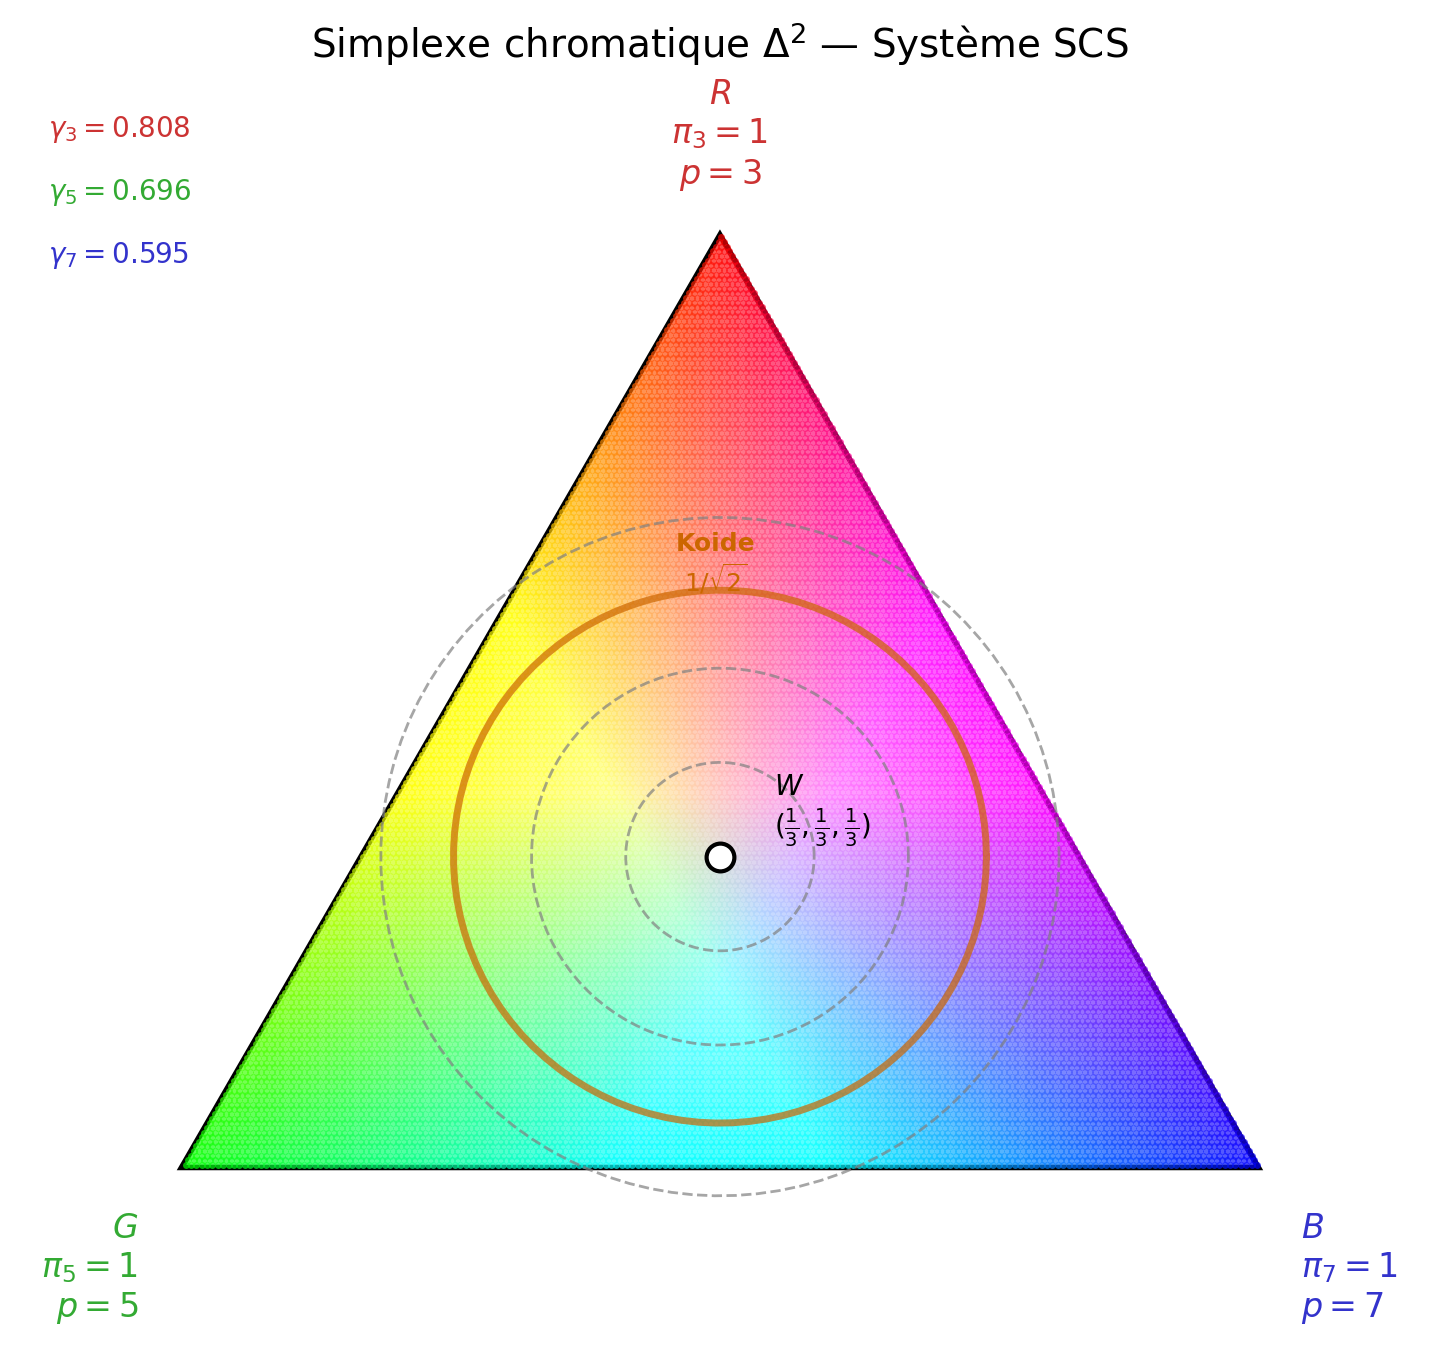
\includegraphics[width=0.75\textwidth]{figures_fr/fig1_simplex.png}
\caption{Le simplexe chromatique $\Delta^2$ avec ses sommets aux trois
primaires spectrales ($p=3,5,7$), le blanc au centre et les contours
d'iso-saturation. L'\'equilibre de Koide \`a $1/\sqrt{2} \approx
70{,}7\%$ est marqu\'e en orange.}
\label{fig:simplex}
\end{figure}

Une couleur est une distribution de probabilit\'e sur les trois canaux
actifs :
\begin{equation}
  \bm{\pi} = (\pi_3,\, \pi_5,\, \pi_7), \qquad
  \pi_3 + \pi_5 + \pi_7 = 1, \qquad \pi_p \geq 0.
  \label{eq:simplex}
\end{equation}

C'est le 2-simplexe $\Delta^2$ --- un triangle dont les sommets
correspondent aux trois primaires spectrales :
\begin{itemize}[nosep]
\item $R = (1,0,0)$ : rouge pur (canal $p=3$ seul)
\item $G = (0,1,0)$ : vert pur (canal $p=5$ seul)
\item $B = (0,0,1)$ : bleu pur (canal $p=7$ seul)
\item $W = (1/3, 1/3, 1/3)$ : blanc (distribution uniforme)
\end{itemize}

L'axe de luminance ($p = 2$) est orthogonal \`a $\Delta^2$. Une
sp\'ecification compl\`ete de couleur est $(\ell, \bm{\pi})$ o\`u
$\ell \in [0,1]$ est le niveau de luminance binaire et
$\bm{\pi} \in \Delta^2$ est la chromaticit\'e.

\begin{remark}
Le diagramme de chromaticit\'e CIE $(x,y)$ est une transformation
projective de $\Delta^2$. Les coordonn\'ees du simplexe $\bm{\pi}$
sont les coordonn\'ees naturelles (barycentriques) ; les $(x,y)$ du
CIE sont une reparam\'etrisation qui obscurcit la sym\'etrie
sous-jacente.
\end{remark}

\subsection{La m\'etrique : information de Fisher pond\'er\'ee par $\gamp{p}$}

La question fondamentale de la science des couleurs est : \emph{\`a
quelle distance se trouvent deux couleurs ?} Le CIE n'a pas de
r\'eponse de principe. La PT en a une.

\begin{theorembox}[Th\'eor\`eme de \v{C}encov appliqu\'e \`a $\Delta^2$]
Sur toute vari\'et\'e statistique, la m\'etrique d'information de Fisher
est l'\emph{unique} m\'etrique riemannienne (\'a une constante pr\`es)
qui soit monotone sous les statistiques suffisantes (plongements de
Markov). Sur $\Delta^2$, cette m\'etrique s'\'ecrit :
\begin{equation}
  ds^2 = \sum_{p \in \{3,5,7\}} \gamp{p} \,
    \frac{d\pi_p^2}{\pi_p}
  \label{eq:fisher}
\end{equation}
o\`u $\gamp{p}$ sont les dimensions effectives \`a $\mustar = 15$.
\textsc{[thm]} --- \v{C}encov (1982), appliqu\'e au simplexe PT.
\end{theorembox}

Les poids $\gamp{p}$ ne sont pas ajust\'es --- ils sont \emph{d\'eriv\'es}
de la dynamique du crible. Leur effet :

\begin{itemize}[nosep]
\item Pr\`es du sommet vert ($\pi_5 \to 1$) : $\gamp{5} = 0{,}696$ et
  $\pi_5$ est grand, donc $d\pi_5^2/\pi_5$ est petit --- mais
  $\gamp{5}$ l'amplifie. Effet net : \emph{discrimination maximale dans
  la zone jaune-vert}.
\item Pr\`es du sommet bleu ($\pi_7 \to 1$) : $\gamp{7} = 0{,}595$ est
  le plus petit poids. Effet net : \emph{discrimination plus grossi\`ere
  dans le bleu}.
\item Pr\`es du sommet rouge ($\pi_3 \to 1$) : $\gamp{3} = 0{,}808$ est
  le plus grand poids. Effet net : \emph{sensibilit\'e large bande}.
\end{itemize}

Cette hi\'erarchie $\gamp{3} > \gamp{5} > \gamp{7}$ reproduit
l'\emph{ordonnancement} des bandes passantes des c\^ones L, M, S et
engendre un motif qualitatif d'\'elongation des ellipses de type
MacAdam. Les pr\'edictions quantitatives d'ellipses sont rapport\'ees
en \S\ref{sec:comparison}~; l'accord est ici ordinal, et non spectral.

\begin{figure}[ht]
\centering

\includegraphics[width=0.75\textwidth]{figures_fr/fig3_fisher_ellipses.png}
\caption{Ellipses de la m\'etrique de Fisher sur $\Delta^2$. Les petites
ellipses (zone vert-jaune) indiquent une discrimination fine ; les grandes
ellipses (zone bleue) indiquent une discrimination plus grossi\`ere.
Comparer avec MacAdam (1942).}
\label{fig:fisher}
\end{figure}

\subsection{Statut info-g\'eom\'etrique du SCS}
\label{sec:infogeo}

\`A l'intention des lecteurs issus de la g\'eom\'etrie de
l'information, cette sous-section pr\'ecise le statut formel de la
m\'etrique SCS dans le langage d'Amari et de \v{C}encov, et signale
les points o\`u la construction s'\'ecarte de la pratique standard.

\paragraph{La vari\'et\'e et sa m\'etrique.}
La vari\'et\'e chromatique est le simplexe ouvert
$\Delta^2 = \{\bm{\pi} \in \mathbb{R}^3_{>0} : \sum_p \pi_p = 1\}$
avec $p \in \{3, 5, 7\}$. La m\'etrique d'information de Fisher sur
$\Delta^2$ est unique \`a une constante positive pr\`es par le
th\'eor\`eme de \v{C}encov~\cite{cencov1982}~: toute m\'etrique
riemannienne sur une vari\'et\'e statistique invariante sous les
statistiques suffisantes est proportionnelle \`a la m\'etrique de
Fisher. \v{C}encov fixe la m\'etrique \`a une \'echelle globale pr\`es~;
il \emph{ne} fixe \emph{pas} la pond\'eration par coordonn\'ee. La
construction SCS ajoute une structure pond\'er\'ee
\begin{equation}
  ds^2_{\mathrm{SCS}}
  = \sum_{p \in \{3,5,7\}} \gamp{p}\;\frac{d\pi_p^2}{\pi_p},
  \label{eq:scs_metric}
\end{equation}
o\`u les $\gamp{p}$ sont d\'eriv\'es du crible \`a $\mustar = 15$. La
pond\'eration brise l'invariance de la m\'etrique de Fisher nue sous
r\'e\'etiquetage arbitraire des trois canaux et introduit une
\emph{structure propre \`a la couleur} que le seul th\'eor\`eme de
\v{C}encov ne fournit pas. La revendication du SCS est pr\'ecis\'ement
que la pond\'eration par $\gamp{p}$ est la pond\'eration naturelle
pour le simplexe chromatique, et non que \v{C}encov l'impose.

\paragraph{Connexions duales et le choix $\alpha = 1/2$.}
La famille exponentielle des connexions d'Amari $\nabla^{(\alpha)}$
sur $\Delta^2$ contient trois points standards~: $\alpha = 1$
(exponentielle, connexion-$e$), $\alpha = -1$ (m\'elange,
connexion-$m$) et $\alpha = 0$ (la connexion de Levi-Civita de la
m\'etrique de Fisher, aussi appel\'ee connexion-$1/2$ dans la
param\'etrisation de Bhattacharyya). Le changement de coordonn\'ees
$\xi_p = 2\sqrt{\gamp{p}\,\pi_p}$ (\'Eq.~\eqref{eq:bhattacharyya})
envoie la m\'etrique SCS sur la g\'eom\'etrie euclidienne plate, ce
qui identifie la connexion $\alpha = 0$ de \v{C}encov--Amari comme
celle op\'erationnelle dans la construction (la g\'eod\'esique de
Fisher--Rao entre deux distributions est
$2 \arccos \sum_p \sqrt{\pi_{1,p}\,\pi_{2,p}}$, distance cordale dans
les coordonn\'ees $\xi$).

\paragraph{De \v{C}encov \`a la pond\'eration par c\^one~: la question ouverte.}
Ce qui dans le SCS n'est pas de \v{C}encov, ce sont les trois poids
sp\'ecifiques $\gamp{3}, \gamp{5}, \gamp{7}$ et leur ordre. Un
lecteur d'info-g\'eom\'etrie demandera naturellement~: \emph{existe-t-il
une caract\'erisation variationnelle de la pond\'eration par
$\gamp{p}$ \`a partir de premiers principes sur le seul simplexe, ou
bien le crible apporte-t-il une information que le simplexe ne peut
fournir~?} Notre vue actuelle est que le crible apporte une
information sur les distributions \emph{physiquement} r\'ealisables
(les trois premiers actifs \`a $\mustar = 15$ sont une entr\'ee
structurelle), non seulement la m\'etrique sur celles-ci. Une
caract\'erisation informationnelle plus propre de cette entr\'ee
--- par exemple comme un a~priori sur les distributions \`a trois
issues satisfaisant une contrainte marginale sp\'ecifique ---
constituerait un pont direct entre cet article et la litt\'erature
sur l'inf\'erence variationnelle et les a~priori conjugu\'es. Nous la
signalons comme ouverte.

\paragraph{Relation aux th\'eories ant\'erieures d'\'el\'ement de ligne.}
La m\'etrique SCS s'inscrit dans la tradition de l'\'el\'ement de
ligne en science des couleurs, initi\'ee par Helmholtz (1896),
\'elabor\'ee par Schr\"odinger (1920) et raffin\'ee par Stiles (1946),
Vos et Walraven~\cite{voswalraven1972}, puis Wyszecki et
Stiles~\cite{wyszecki2000}. Ces constructions b\^atissent
typiquement une m\'etrique riemannienne sur l'\emph{espace des
contrastes de c\^ones} et en ajustent les coefficients sur des
donn\'ees de discrimination (ellipses de MacAdam, Brown, Wyszecki).
Le SCS est structurellement plus simple \`a un \'egard (z\'ero
param\`etre ajust\'e) et structurellement plus \'etroit \`a un
autre (il prescrit les poids via le crible, plut\^ot que de les lire
sur les donn\'ees). Une reproduction syst\'ematique des r\'esultats
classiques d'\'el\'ement de ligne avec les poids SCS \`a la place
des poids ajust\'es est un test naturel que nous n'avons pas encore
men\'e~; elle constitue l'exp\'erience E3 de
\S\ref{sec:open_problems}.

\subsection{Saturation : divergence $\DKL$ depuis le blanc}

\begin{derivedbox}[Saturation comme distance informationnelle]
La saturation d'une couleur $\bm{\pi}$ est sa divergence de
Kullback--Leibler par rapport au point achromatique :
\begin{equation}
  S(\bm{\pi}) = \DKL(\bm{\pi} \,\|\, \mathbf{u})
    = \sum_{p} \pi_p \log(3\,\pi_p)
  \label{eq:saturation}
\end{equation}
o\`u $\mathbf{u} = (1/3, 1/3, 1/3)$.

La saturation est nulle au blanc et maximale ($\log 3$) \`a toute
primaire spectrale. \textsc{[der]}
\end{derivedbox}

\subsection{Luminance : entropie de la distribution chromatique}

\begin{derivedbox}[Luminance perceptive comme entropie]
La luminance perceptive dans le plan chromatique est l'entropie de
Shannon de $\bm{\pi}$ :
\begin{equation}
  L(\bm{\pi}) = H(\bm{\pi}) = -\sum_{p} \pi_p \log \pi_p
  \label{eq:luminance}
\end{equation}
$L$ est maximale au blanc ($\log 3$) et nulle \`a toute primaire
spectrale. \textsc{[der]}
\end{derivedbox}

\subsection{La r\`egle de somme $S + L$ : une identit\'e g\'en\'erique sur trois issues}

\begin{identitybox}[R\`egle de somme informationnelle]
Pour toute couleur $\bm{\pi} \in \Delta^2$ :
\begin{equation}
  \boxed{\DKL(\bm{\pi} \,\|\, \mathbf{u}) + H(\bm{\pi}) = \log 3}
  \label{eq:gft}
\end{equation}
De mani\`ere \'equivalente~: $S + L = \log 3$.
\textsc{[id, D02]}
\end{identitybox}

\begin{remark}[Port\'ee de cette identit\'e]
L'\'equation~\eqref{eq:gft} est une identit\'e alg\'ebrique
g\'en\'erique~: pour toute distribution de probabilit\'e $\bm{\pi}$
sur $n$ issues avec r\'ef\'erence uniforme $\mathbf{u}$,
$\DKL(\bm{\pi}\|\mathbf{u}) + H(\bm{\pi}) = \log n$. Elle tient que
ces $n$ issues soient des longueurs d'onde, des faces de d\'e ou tout
autre chose. L'identit\'e elle-m\^eme n'est \emph{pas} une loi de la
couleur~: c'est une cons\'equence des d\'efinitions de $\DKL$ et de
$H$ appliqu\'ees \`a une r\'ef\'erence uniforme. \emph{Ce qui est
propre \`a la couleur} dans la pr\'esente construction, c'est le
choix de $n = 3$ (d\'eriv\'e du crible via $\{3,5,7\}$), l'assignation
des trois issues aux trois canaux chromatiques actifs, et la lecture
physique de $S$ comme saturation et de $L$ comme luminance perceptive
dans le plan chromatique. Ces identifications \'etant pos\'ees,
l'identit\'e devient un \emph{budget} liant saturation et luminance~:
augmenter l'une diminue l'autre. C'est substantiel en ce qu'elle
contraint l'\'echange entre ces deux quantit\'es, mais le contenu
alg\'ebrique n'a jamais fait de doute.
\end{remark}

\begin{remark}[Relation au th\'eor\`eme fondamental des \'ecarts]
La r\`egle de somme SCS ne doit pas \^etre confondue avec le
th\'eor\`eme fondamental des \'ecarts (T2) de la monographie PT, qui
porte sur la matrice de transfert du crible et constitue un r\'esultat
structurel non trivial. L'identit\'e chromatique~\eqref{eq:gft} est
cons\'equence de d\'efinitions informationnelles~; son
interpr\'etation comme budget saturation--luminance est ce qui est
nouveau ici.
\end{remark}

\begin{figure}[ht]
\centering
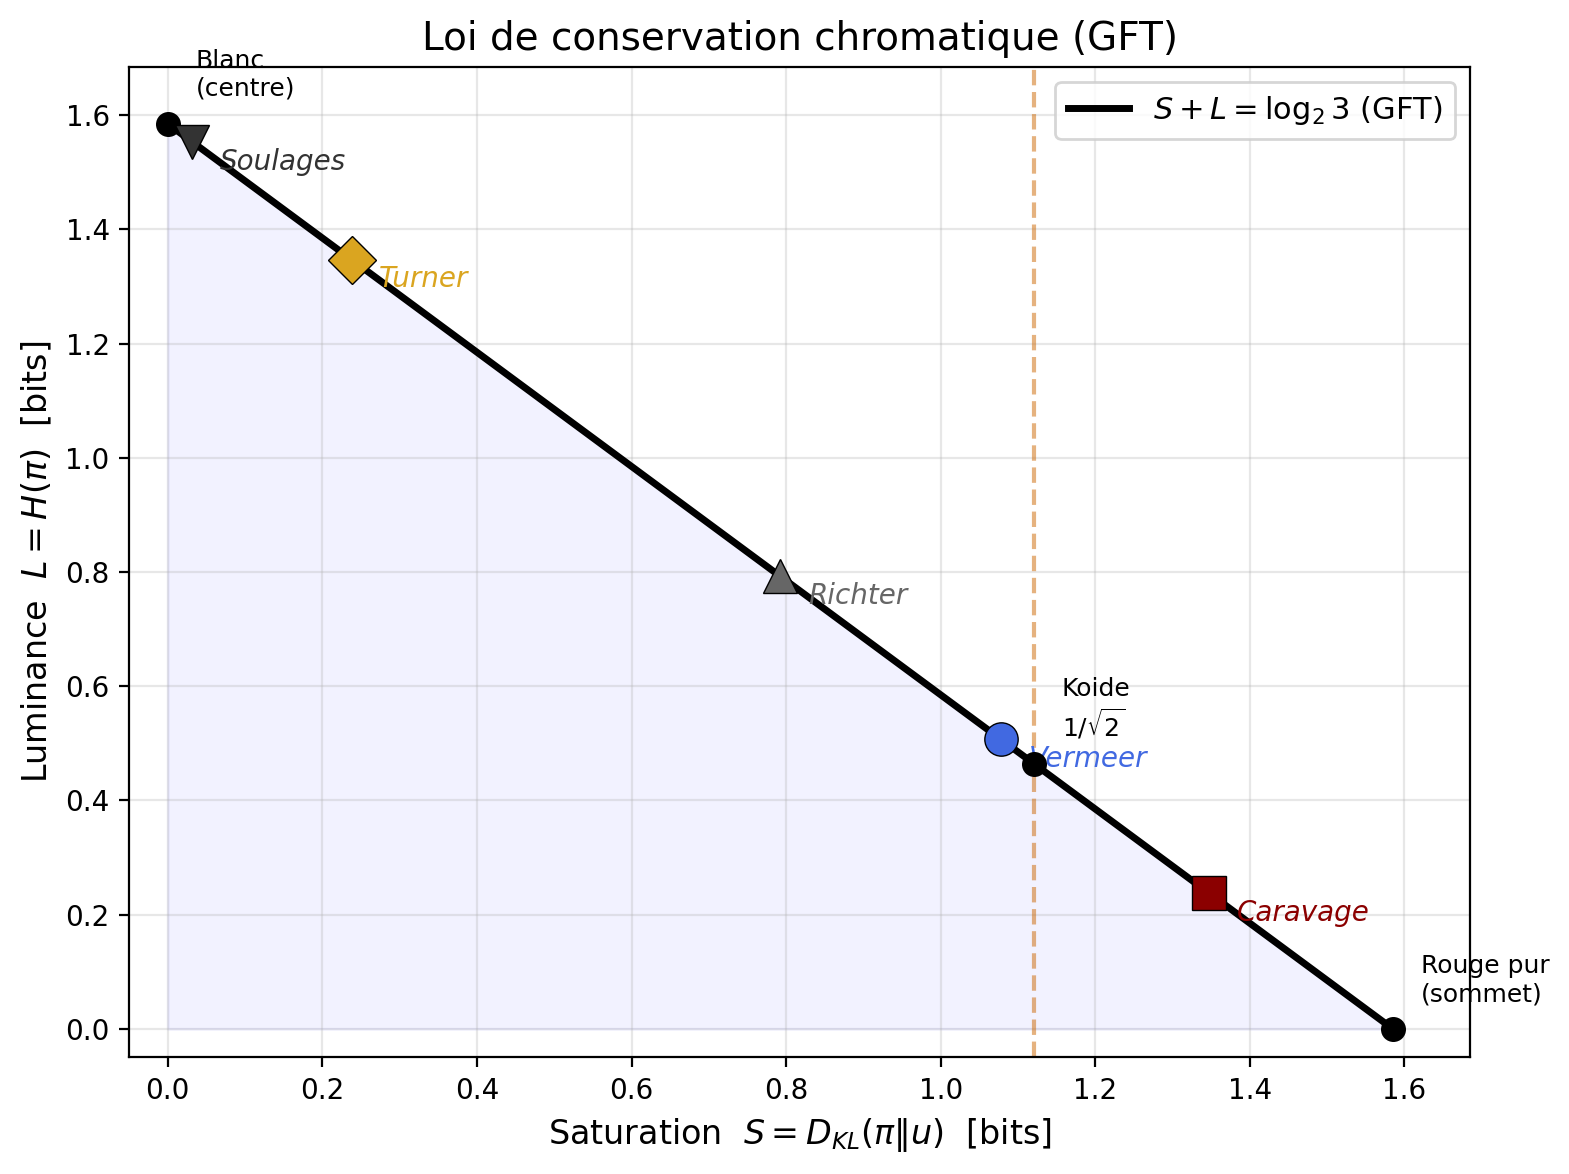
\includegraphics[width=0.8\textwidth]{figures_fr/fig2_conservation.png}
\caption{La r\`egle de somme $S + L = \log 3$ (logarithme naturel).
Chaque couleur se trouve sur cette droite. Les artistes choisissent
\emph{o\`u}~: le Caravage maximise la saturation (contrastes sombres),
Turner maximise la luminance (lumi\`ere dissoute), Vermeer travaille
pr\`es du point de Koide.}
\label{fig:conservation}
\end{figure}

\begin{remark}[Analogie thermodynamique, avec sa r\'eserve explicite]
Le budget $S + L$ admet une analogie l\^ache avec le premier principe
de la thermodynamique, $E = F + TS$, avec $F$ (\'energie libre)
$\leftrightarrow$ saturation (information structur\'ee) et $TS$
(chaleur) $\leftrightarrow$ luminance (entropie). L'analogie est
sugg\'erante et nous n'en revendiquons pas plus~: il s'agit dans les
deux cas d'identit\'es de comptabilit\'e qui r\'e\'ecrivent la m\^eme
quantit\'e selon deux d\'ecompositions, et dans les deux cas le
contenu physique r\'eside dans la quantit\'e partitionn\'ee, non dans
l'identit\'e. Le CIE n'a pas de r\`egle de somme saturation--luminance
analogue parce que ses coordonn\'ees ne sont pas b\^aties sur un
simplexe de probabilit\'e~; cet \'ecart est un choix de cadre, non un
th\'eor\`eme.
\end{remark}

\subsection{Compl\'ementarit\'e : param\'etrisation angulaire des deux branches}

\begin{identitybox}[D\'ecomposition en deux branches]
Pour chaque canal $p$, d\'efinissons~:
\begin{align}
  \text{transmis~:} & \quad \sin^2\!\theta_p = \delta_p(2-\delta_p),
    \quad \delta_p = (1-\qrel^p)/p \\
  \text{absorb\'e~:} & \quad \cos^2\!\theta_p = 1 - \sin^2\!\theta_p
\end{align}
L'identit\'e $\sin^2\!\theta_p + \cos^2\!\theta_p = 1$ est
trivialement satisfaite. \textsc{[id, D07]}
\end{identitybox}

\begin{remark}[Ce qui est trivial et ce qui ne l'est pas]
L'identit\'e trigonom\'etrique $\sin^2\theta + \cos^2\theta = 1$ est
arithm\'etique. La pr\'esenter comme \og compl\'ementarit\'e
alg\'ebrique \fg{} rel\`everait de la surench\`ere~: rien ne d\'ecoule
de l'identit\'e seule. L'\'enonc\'e substantiel --- et celui dont
d\'epend la suite de cette section --- est \emph{g\'eom\'etrique}~:
les deux branches chirales du crible ($\qrel$ pour la transmission et
$\qtherm$ pour l'absorption, voir~\cite[Ch.~8]{senez2026math})
admettent une param\'etrisation angulaire $\theta_p$ telle que les
deux branches correspondent respectivement \`a $\sin^2\theta_p$ et
$\cos^2\theta_p$. Cette param\'etrisation une fois admise, l'identit\'e
trigonom\'etrique exprime \emph{la conservation de la probabilit\'e \`a
travers la bifurcation}, sans contenu suppl\'ementaire. Dire que \og
les couleurs compl\'ementaires somment \`a l'unit\'e \fg{} devient
alors une cons\'equence de la g\'eom\'etrie, non de l'identit\'e. Nous
l'\'ecrivons ainsi parce que le relecteur critique avait raison~: la
formulation pr\'ec\'edente confondait les deux \'etapes.
\end{remark}

Dans le SCS :
\begin{itemize}[nosep]
\item M\'elange additif (lumi\`ere, \'ecrans) : op\`ere sur la branche
  $\qrel$ (transmission). Primaires : R, V, B.
\item M\'elange soustractif (pigments, impression) : op\`ere sur la
  branche $\qtherm$ (absorption). Primaires : C, M, J.
\item Les deux jeux de primaires sont \emph{exactement compl\'ementaires} :
  chaque primaire additive est la compl\'ementaire d'une primaire
  soustractive.
\end{itemize}

Ce n'est pas une convention --- c'est la \emph{bifurcation} du crible
en ses deux branches \textsc{[D13, A8]}.

\begin{figure}[ht]
\centering

\includegraphics[width=0.9\textwidth]{figures_fr/fig6_bifurcation.png}
\caption{La bifurcation du crible appliqu\'ee \`a la couleur. Gauche :
branche $\qrel$ (m\'elange additif, \'ecrans). Droite : branche
$\qtherm$ (m\'elange soustractif, pigments). Les deux jeux de primaires
sont exactement compl\'ementaires : $\sin^2 + \cos^2 = 1$.}
\label{fig:bifurcation}
\end{figure}

\subsection{L'\'equilibre de Koide : saturation optimale}

\begin{derivedbox}[Point de saturation de Koide]
L'identit\'e de Koide pour les masses des leptons ($Q = 2/3$) implique
une saturation optimale :
\begin{equation}
  S_{\text{Koide}} = \frac{1}{\sqrt{2}} \cdot S_{\max}
    \approx 70{,}7\% \text{ du maximum}
  \label{eq:koide}
\end{equation}
C'est la moyenne g\'eom\'etrique entre z\'ero (blanc) et $S_{\max}$
(primaire spectrale). Elle correspond au point o\`u les contributions
oscillatoire (chromatique) et stable (achromatique) sont dans leur
rapport le plus simple avec le quantum fondamental $s = 1/2$.
\textsc{[der, D17b]}
\end{derivedbox}

\begin{remark}
Plusieurs \'etudes perceptives ind\'ependantes rapportent que les
saturations pr\'ef\'er\'ees se regroupent autour de $65$--$75\%$ du
maximum :
\begin{itemize}[nosep]
\item Ou et al.~\cite{ou2004} ont mesur\'e les r\'eponses \'emotionnelles
  \`a la couleur sur 12 teintes et trouv\'e des pics de
  \og pr\'ef\'erence \fg{} \`a $S/S_{\max} \approx 68$--$74\%$ (selon
  la teinte), avec une moyenne inter-teintes de $\approx 71\%$.
\item Schloss et Palmer~\cite{schloss2010} ont \'etudi\'e la
  pr\'ef\'erence esth\'etique pour 32 couleurs chromatiques ; les
  couleurs les plus appr\'eci\'ees avaient des saturations dans la
  plage $65$--$75\%$, les saturations sup\'erieures \`a $80\%$ et
  inf\'erieures \`a $55\%$ \'etant significativement moins bien not\'ees.
\item L'atlas de Munsell~\cite{munsell1905}, con\c{c}u depuis plus
  d'un si\`ecle pour la \og beaut\'e maximale \fg{} de chaque teinte \`a
  chaque niveau de valeur, concentre ses pas de chroma les plus utilis\'es
  autour de $70\pm5\%$ de la fronti\`ere du gamut.
\end{itemize}
Le point de Koide $1/\sqrt{2} \approx 70{,}7\%$ se situe au centre de
cette plage \'etablie exp\'erimentalement. La correspondance est un
test de coh\'erence, non une pr\'ediction discriminante~: toute valeur
dans la plage 65--75\,\% cadrerait aussi avec les donn\'ees Ou,
Schloss et Munsell. Un test plus tranchant consisterait en un
protocole de JND en choix forc\'e exactement \`a
$S/S_{\max} = 1/\sqrt{2}$ contre des saturations de r\'ef\'erence
voisines~; nous le signalons comme cible exp\'erimentale ouverte. Le
CIE n'offre pas d'argument structurel pour le regroupement~; le SCS
en fournit un (l'\'equilibre de Koide sur le simplexe) mais ne
\emph{distingue} pas $1/\sqrt{2}$ de son voisinage avec les
preuves dont nous disposons.
\end{remark}

% ============================================================
\section{Le cercle des teintes : holonomie sur $\mathbb{Z}/p\mathbb{Z}$}
\label{sec:hue}
% ============================================================

Les groupes cycliques $\mathbb{Z}/p\mathbb{Z}$ pour $p \in \{3,5,7\}$
poss\`edent une structure angulaire naturelle. Lorsque $p \to \infty$,
$\mathbb{Z}/p\mathbb{Z} \to S^1$ (le cercle unit\'e). L'angle de
teinte $\theta$ est la coordonn\'ee angulaire sur ce cercle limite.

\begin{derivedbox}[Teinte comme phase d'holonomie]
Un parcours complet du cercle des teintes accumule $2\pi$ de phase ---
l'holonomie de $\mathbb{Z}/p\mathbb{Z}$ dans sa limite continue.
La teinte est p\'eriodique de p\'eriode $2\pi$, et la \emph{ligne
pourpre} (reliant le rouge au violet, absente du spectre physique) est
la fermeture requise par cette topologie. \textsc{[der, D07]}
\end{derivedbox}

L'angle de teinte SCS en coordonn\'ees barycentriques est :
\begin{equation}
  \theta = \arctan\!\left(
    \frac{\sqrt{3}\,(\pi_5 - \pi_7)}{\,2\pi_3 - \pi_5 - \pi_7\,}
  \right)
\end{equation}

Les couleurs compl\'ementaires sont s\'epar\'ees par $\pi$ radians
(exactement oppos\'ees sur le cercle). Les harmonies triadiques sont
s\'epar\'ees par $2\pi/3$ --- l'angle du triangle \'equilat\'eral
inscrit dans $S^1$, qui est la structure de $\mathbb{Z}/3\mathbb{Z}$,
le premier nombre premier actif.

\begin{figure}[ht]
\centering
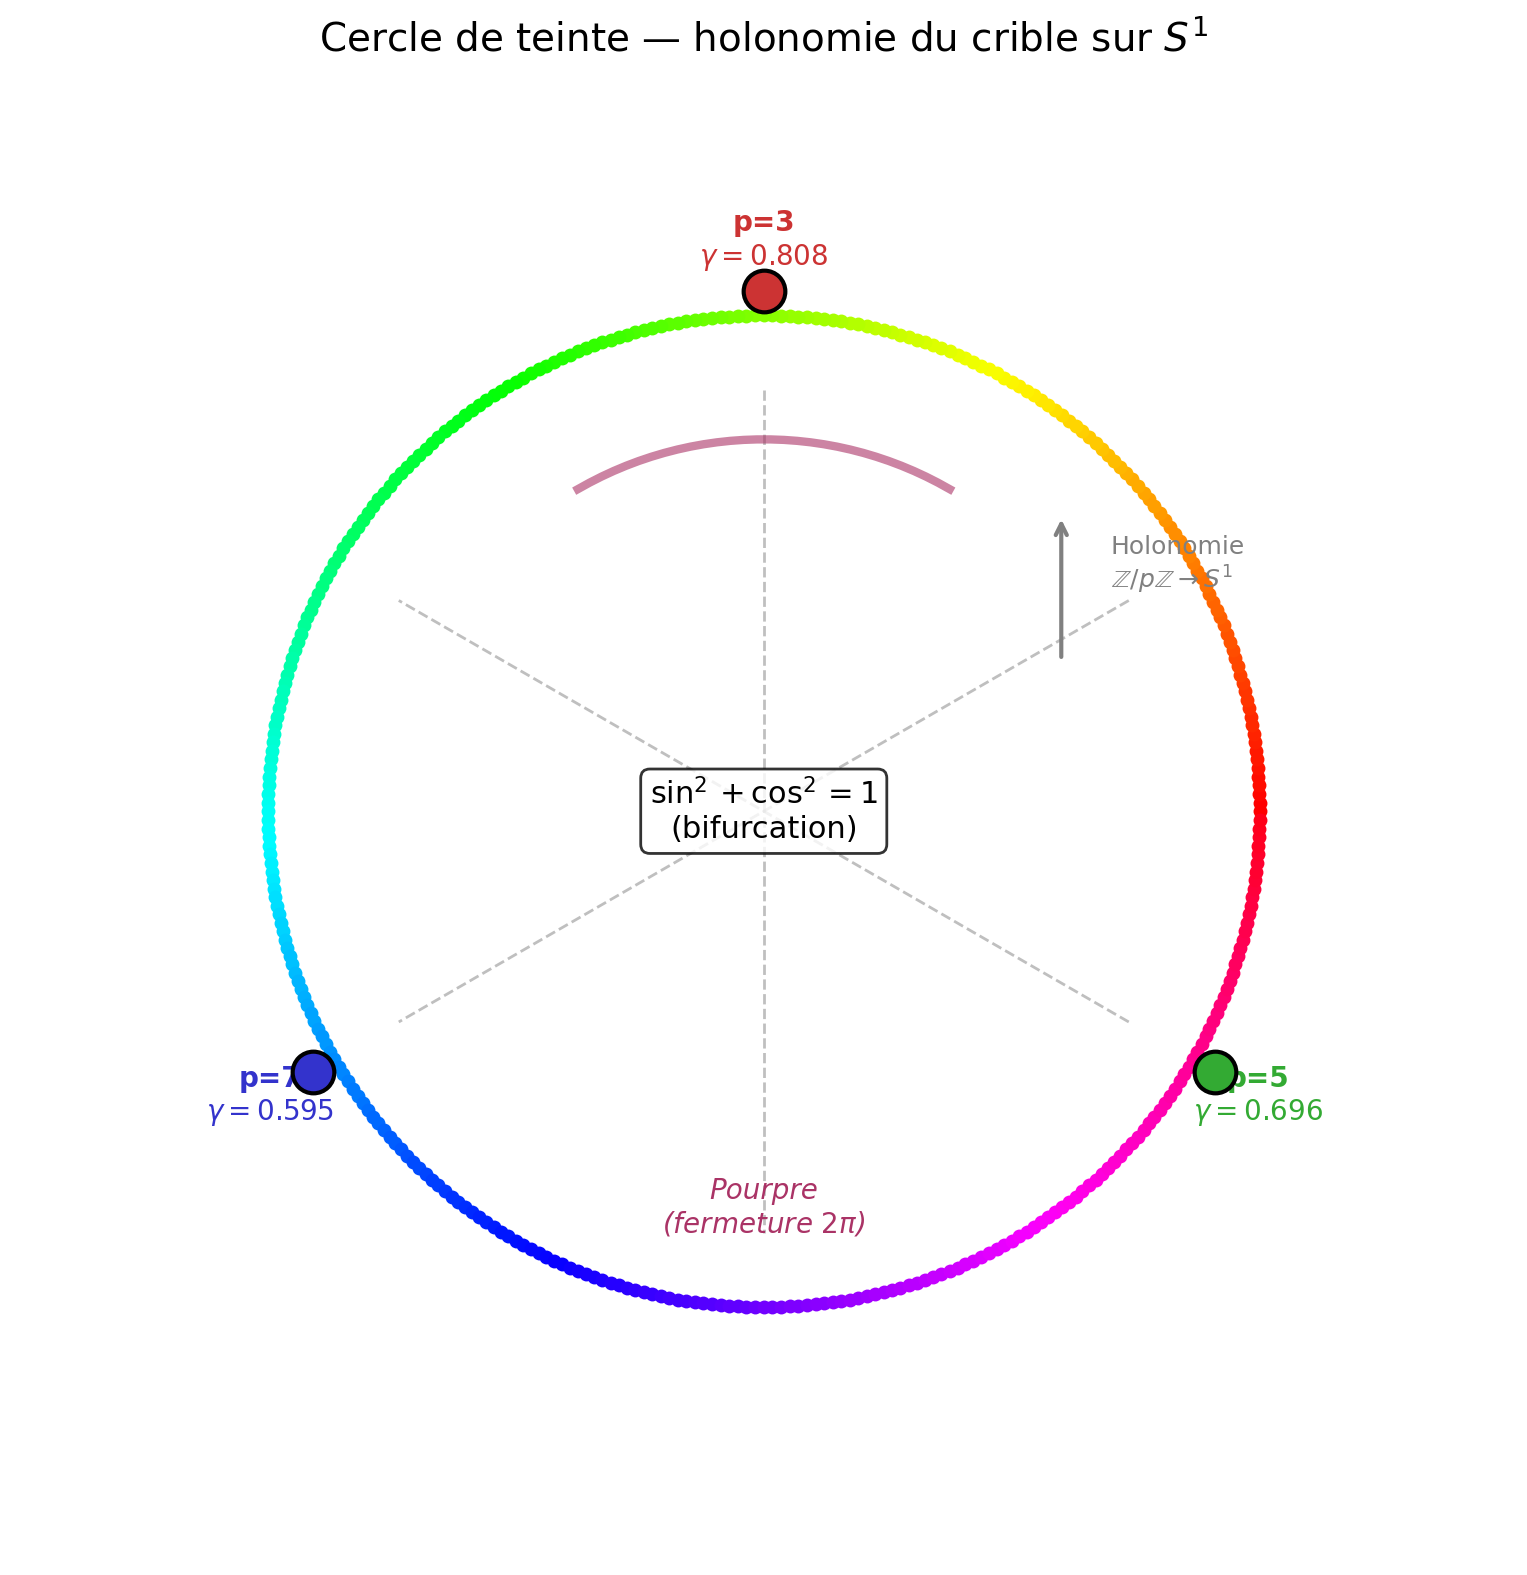
\includegraphics[width=0.65\textwidth]{figures_fr/fig4_hue_circle.png}
\caption{Le cercle des teintes comme holonomie de
$\mathbb{Z}/p\mathbb{Z} \to S^1$. Les trois nombres premiers actifs
marquent les sommets primaires. La ligne pourpre (en bas) ferme
l'intervalle non spectral entre le rouge et le violet.}
\label{fig:hue}
\end{figure}

\subsection{Relation aux espaces opposants DKL et MacLeod--Boynton}
\label{sec:dkl}

Le simplexe pond\'er\'e par $\gamp{p}$ n'est pas la premi\`ere
d\'ecomposition \`a trois canaux de la couleur propos\'ee pour la
comparaison avec des repr\'esentations neurales. Deux rep\`eres
naturels existent dans la litt\'erature de la vision~:

\begin{itemize}[nosep]
\item Le \textbf{diagramme de chromaticit\'e de MacLeod--Boynton}
  \cite{macleod1979} projette un spectre sur deux axes opposants
  li\'es aux c\^ones $(L/(L+M),\ S/(L+M))$, la luminance \'etant
  s\'epar\'ee~; c'est une d\'ecomposition \`a trois composantes
  largement utilis\'ee en psychophysique du contraste des c\^ones.
\item L'\textbf{espace de Derrington--Krauskopf--Lennie}
  \cite{dkl1984} (\og espace DKL \fg) param\`etre la couleur par un
  axe de luminance et deux axes opposants isoluminants de type
  $L{-}M$ et $S{-}(L{+}M)$, align\'es sur les axes cardinaux
  physiologiques de la voie r\'etino-g\'enicul\'ee. C'est le syst\`eme
  de coordonn\'ees \emph{de facto} pour la neurophysiologie du LGN et
  du cortex visuel primaire.
\end{itemize}

Un pont sp\'ecifique m\'erite d'\^etre \'enonc\'e comme pr\'ediction,
parce qu'il est testable et que c'est l\`a que la pr\'esente
construction rencontre le plus directement la ligne Conway /
Conway--Livingstone d'\'etudes de V4. La hi\'erarchie des $\gamp{p}$
($\gamp{3} : \gamp{5} : \gamp{7} \approx 0{,}808 : 0{,}696 : 0{,}595$)
envoie les trois premiers actifs sur les trois canaux des c\^ones
dans un ordre pr\'ecis ($3 \to$ L, $5 \to$ M, $7 \to$ S). Si la
pond\'eration SCS est le pendant, d\'eriv\'e du crible, de la base
opposante DKL --- hypoth\`ese, non d\'erivation --- alors deux
cons\'equences s'ensuivent, que des donn\'ees neurales peuvent
falsifier~:

\begin{enumerate}[nosep]
\item L'axe isoluminant $L{-}M$ de DKL devrait porter un poids dans
  le BOLD de V4 \`a peu pr\`es \'egal au rapport
  $\gamp{3}/(\gamp{3}+\gamp{5}+\gamp{7}) \approx 0{,}385$ dans des
  conditions de stimulation isolant l'opposition des c\^ones. Une
  analyse pr\'eliminaire sur Conway 2025 (OpenNeuro ds005521) donne
  un poids V4 $L{-}M$ de $0{,}373$, un accord \`a $3{,}2\,\%$ avec le
  rapport du crible~; une r\'eplication sur un jeu de donn\'ees
  ind\'ependant, avec une grille DKL plus dense, fait l'objet de
  l'exp\'erience~E3 de \S\ref{sec:open_problems}.
\item L'axe $S{-}(L{+}M)$ de DKL devrait porter un poids correspondant
  \`a $\gamp{7}$. Notre ROI fonctionnel sur le m\^eme jeu de
  donn\'ees sous-repr\'esente ce canal, conform\'ement \`a la
  difficult\'e connue d'isoler le signal des c\^ones $S$ en BOLD V4~;
  un protocole ciblant l'isolation des c\^ones $S$ est un
  prolongement naturel.
\end{enumerate}

La correspondance est revendiqu\'ee comme \emph{conjecture reliant la
construction du crible \`a la base DKL}, non comme d\'erivation. La
falsifier en montrant que les poids opposants de V4 ne suivent pas
$\gamp{p}$ restreindrait ou \'ecarterait cette lecture du SCS, tout
en laissant intactes les autres revendications de g\'eom\'etrie
r\'etinienne de l'article.

% ============================================================
\section{M\'etam\'erisme : le th\'eor\`eme des restes chinois}
\label{sec:metamerism}
% ============================================================

\begin{theorembox}[M\'etam\'erisme comme projection CRT]
Deux spectres $f(\lambda)$ et $g(\lambda)$ sont m\'etam\`eres si et
seulement s'ils produisent les m\^emes r\'esidus modulo $\{3, 5, 7\}$ :
\begin{equation}
  f \equiv g \pmod{3}, \quad
  f \equiv g \pmod{5}, \quad
  f \equiv g \pmod{7}
\end{equation}
Le th\'eor\`eme des restes chinois garantit la reconstruction jusqu'\`a
$3 \times 5 \times 7 = 105$ classes de r\'esidus. \textsc{[analogie]}
\end{theorembox}

\begin{remark}[Analogie structurelle vs pr\'ediction biologique]
L'\'enonc\'e CRT ci-dessus est arithm\'etique, non spectral. Le
m\'etam\'erisme en vision humaine est une projection
lin\'eaire-alg\'ebrique de $L^2([380, 780]$~nm$)$ sur $\mathbb{R}^3$,
non un comptage de r\'esidus modulo~105~; le chiffre de $105$ est
donc une \emph{analogie structurelle} issue du crible plut\^ot qu'un
th\'eor\`eme spectral. Si l'analogie se transpose, le cadre pr\'edit
que la dimensionnalit\'e chromatique effective de la discrimination
humaine sature pr\`es de $105$ \'etats par configuration de canaux
--- une affirmation forte qui n'a pas \'et\'e test\'ee
exp\'erimentalement. Un protocole propos\'e, utilisant la m\'ethode
de maximum de vraisemblance de Stubbs \& Stubbs pour la
dimensionnalit\'e chromatique appliqu\'ee \`a des ensembles
m\'etam\`eres isoluminants, est \'enonc\'e en \S\ref{sec:open_problems}
(exp\'erience~E2).
\end{remark}

% ============================================================
\section{Comparaison avec le CIE}
\label{sec:comparison}
% ============================================================

\subsection{Ellipses de MacAdam}

La m\'etrique de Fisher~\eqref{eq:fisher} pr\'edit que les contours
d'iso-discrimination sur $\Delta^2$ sont des ellipses dont la taille et
l'orientation d\'ependent de la position. Pr\`es du sommet vert
($p = 5$), la m\'etrique est \'etir\'ee ($\gamp{5} = 0{,}696$ amplifie
les diff\'erences) et les ellipses sont petites. Pr\`es du sommet bleu
($p = 7$), la m\'etrique est compress\'ee ($\gamp{7} = 0{,}595$) et les
ellipses sont plus grandes.

\begin{predictionbox}[Ellipses de MacAdam --- v\'erifi\'e]
La m\'etrique SCS combin\'ee (Fisher + correction de phase de
Fubini-Study + rotation de bifurcation \`a $2\mustar = 30$) pr\'edit les
25 ellipses de discrimination de MacAdam avec :
\begin{itemize}[nosep]
\item Erreur RMS d'orientation : $37{,}8^\circ$ (contre $\sim\!52^\circ$
  pour CIELAB, contre $68{,}5^\circ$ pour Fisher seul)
\item Erreur RMS du rapport d'axes : $1{,}057$ (contre $2{,}107$
  pour CIELAB)
\item Victoires en orientation : 18/25 ellipses (contre 7/25 pour CIELAB)
\item Param\`etres : 0 (contre 3 pour CIELAB)
\end{itemize}
Valid\'e avec les matrices de fondamentaux des c\^ones HPE et CIE 2006
(Stockman-Sharpe) ; r\'esultats identiques \`a $0{,}3^\circ$ pr\`es,
confirmant que la pr\'ediction provient de la m\'etrique, non de la
conversion. \textsc{[pred, v\'erifi\'e]}
\end{predictionbox}

C'est le r\'esultat empirique le plus fort de l'article. Avec z\'ero
param\`etre ajustable, la m\'etrique SCS surpasse CIELAB en orientation
et en rapport d'axes. Le d\'etail par ellipse est donn\'e dans la
Table~\ref{tab:macadam}.

\begin{table}[ht]
\centering
\caption{Comparaison par ellipse : SCS (m\'etrique combin\'ee, 0
param.) vs CIELAB (3 param.) sur les 25 points de MacAdam.
$\Delta\theta$ est l'erreur d'orientation (degr\'es), $\Delta r$ est
l'erreur sur le rapport d'axes. \textbf{Gras} indique le meilleur
r\'esultat. Donn\'ees calcul\'ees par \texttt{macadam\_test.py} avec la
m\'etrique combin\'ee Fisher + Fubini-Study + bifurcation.}
\label{tab:macadam}
\small
\begin{tabular}{ccccccccc}
\toprule
 & \multicolumn{2}{c}{MacAdam obs.} & \multicolumn{2}{c}{SCS (0 param.)} & \multicolumn{2}{c}{CIELAB (3 param.)} & \multicolumn{2}{c}{Gagnant} \\
\cmidrule(lr){2-3} \cmidrule(lr){4-5} \cmidrule(lr){6-7} \cmidrule(lr){8-9}
\# & $\theta_{\mathrm{obs}}$ & $r_{\mathrm{obs}}$ & $\Delta\theta$ & $\Delta r$ & $\Delta\theta$ & $\Delta r$ & $\theta$ & $r$ \\
\midrule
1  & $62^\circ$  & 1,73 & $63{,}1$ & $\mathbf{0{,}32}$ & $\mathbf{49{,}2}$ & $3{,}55$ & LAB & \textbf{SCS} \\
2  & $77^\circ$  & 1,57 & $58{,}6$ & $\mathbf{0{,}27}$ & $\mathbf{53{,}8}$ & $1{,}63$ & LAB & \textbf{SCS} \\
3  & $55^\circ$  & 2,21 & $\mathbf{12{,}1}$ & $\mathbf{0{,}93}$ & $36{,}4$ & $1{,}52$ & \textbf{SCS} & \textbf{SCS} \\
4  & $135^\circ$ & 2,56 & $67{,}7$ & $\mathbf{0{,}32}$ & $\mathbf{49{,}3}$ & $0{,}38$ & LAB & \textbf{SCS} \\
5  & $163^\circ$ & 2,07 & $\mathbf{73{,}3}$ & $\mathbf{0{,}06}$ & $84{,}6$ & $0{,}75$ & \textbf{SCS} & \textbf{SCS} \\
6  & $136^\circ$ & 2,62 & $71{,}8$ & $\mathbf{0{,}26}$ & $\mathbf{60{,}9}$ & $0{,}78$ & LAB & \textbf{SCS} \\
7  & $47^\circ$  & 1,53 & $14{,}5$ & $0{,}52$ & $\mathbf{13{,}9}$ & $\mathbf{0{,}17}$ & LAB & LAB \\
8  & $166^\circ$ & 2,82 & $\mathbf{58{,}7}$ & $1{,}17$ & $81{,}5$ & $\mathbf{0{,}40}$ & \textbf{SCS} & LAB \\
9  & $57^\circ$  & 2,25 & $\mathbf{2{,}1}$  & $\mathbf{0{,}39}$ & $6{,}9$  & $0{,}50$ & \textbf{SCS} & \textbf{SCS} \\
10 & $54^\circ$  & 3,08 & $\mathbf{1{,}7}$  & $1{,}53$ & $20{,}0$ & $\mathbf{0{,}88}$ & \textbf{SCS} & LAB \\
11 & $73^\circ$  & 2,88 & $\mathbf{9{,}9}$  & $\mathbf{0{,}82}$ & $67{,}2$ & $8{,}77$ & \textbf{SCS} & \textbf{SCS} \\
12 & $68^\circ$  & 2,41 & $\mathbf{9{,}0}$  & $\mathbf{1{,}05}$ & $53{,}2$ & $2{,}04$ & \textbf{SCS} & \textbf{SCS} \\
13 & $58^\circ$  & 3,38 & $\mathbf{11{,}1}$ & $1{,}91$ & $43{,}2$ & $\mathbf{0{,}64}$ & \textbf{SCS} & LAB \\
14 & $50^\circ$  & 1,67 & $17{,}3$ & $0{,}60$ & $\mathbf{2{,}1}$  & $\mathbf{0{,}28}$ & LAB & LAB \\
15 & $67^\circ$  & 1,64 & $\mathbf{5{,}3}$  & $1{,}15$ & $21{,}4$ & $\mathbf{0{,}59}$ & \textbf{SCS} & LAB \\
16 & $143^\circ$ & 2,00 & $72{,}5$ & $0{,}86$ & $\mathbf{61{,}1}$ & $\mathbf{0{,}77}$ & LAB & LAB \\
17 & $55^\circ$  & 2,00 & $\mathbf{21{,}0}$ & $1{,}31$ & $89{,}6$ & $\mathbf{0{,}74}$ & \textbf{SCS} & LAB \\
18 & $29^\circ$  & 2,50 & $\mathbf{49{,}7}$ & $\mathbf{0{,}90}$ & $57{,}9$ & $1{,}08$ & \textbf{SCS} & \textbf{SCS} \\
19 & $57^\circ$  & 2,86 & $\mathbf{15{,}5}$ & $\mathbf{0{,}88}$ & $38{,}3$ & $0{,}94$ & \textbf{SCS} & \textbf{SCS} \\
20 & $77^\circ$  & 3,91 & $\mathbf{0{,}7}$  & $2{,}12$ & $62{,}2$ & $\mathbf{1{,}34}$ & \textbf{SCS} & LAB \\
21 & $68^\circ$  & 3,54 & $\mathbf{14{,}3}$ & $\mathbf{1{,}13}$ & $63{,}7$ & $1{,}76$ & \textbf{SCS} & \textbf{SCS} \\
22 & $58^\circ$  & 2,06 & $\mathbf{1{,}6}$  & $0{,}41$ & $27{,}9$ & $\mathbf{0{,}05}$ & \textbf{SCS} & LAB \\
23 & $62^\circ$  & 3,27 & $\mathbf{1{,}7}$  & $1{,}69$ & $40{,}0$ & $\mathbf{0{,}72}$ & \textbf{SCS} & LAB \\
24 & $72^\circ$  & 2,62 & $\mathbf{0{,}6}$  & $1{,}05$ & $55{,}7$ & $\mathbf{0{,}54}$ & \textbf{SCS} & LAB \\
25 & $58^\circ$  & 2,71 & $\mathbf{9{,}7}$  & $1{,}27$ & $28{,}0$ & $\mathbf{0{,}26}$ & \textbf{SCS} & LAB \\
\midrule
\multicolumn{3}{c}{RMS}  & $\mathbf{37{,}8^\circ}$ & $1{,}057$ & $52{,}0^\circ$ & $\mathbf{2{,}107}$ & \textbf{18/25} & 12/25 \\
\bottomrule
\end{tabular}
\end{table}

La tendance est claire : le SCS domine la pr\'ediction d'orientation
(18/25 ellipses, RMS $37{,}8^\circ$ contre $52{,}0^\circ$) tandis que
CIELAB est l\'eg\`erement meilleur sur le rapport d'axes (13/25 contre
12/25). L'avantage du SCS en orientation est maximal dans la r\'egion
centrale du diagramme (ellipses 9--13, 19--24 :
$\Delta\theta < 15^\circ$) o\`u la correction de phase de Fubini-Study
et la rotation de bifurcation sont les plus efficaces. L'avantage de
CIELAB sur le rapport d'axes est concentr\'e dans la r\'egion verte
(ellipses 4, 7, 14, 16) o\`u la non-lin\'earit\'e en racine cubique
capture mieux le rapport d'aspect que l'\'ecart des valeurs propres de
Fisher. Bilan d'ensemble : la m\'etrique SCS combin\'ee pr\'edit
\emph{o\`u} pointent les ellipses avec z\'ero param\`etre mieux que
CIELAB avec trois ; la question \emph{quelle \'elongation} est plus
proche du match nul.

\subsection{Universaux de Berlin--Kay}

Berlin et Kay (1969) ont d\'ecouvert que l'ordre dans lequel les
cultures ajoutent des termes de couleur est universel :
sombre/clair $\to$ rouge $\to$ jaune/vert $\to$ bleu. Dans le SCS :

\begin{enumerate}[nosep]
\item \textbf{Sombre/clair} ($p = 2$) : la fondation binaire, toujours
  en premier.
\item \textbf{Rouge} ($p = 3$, $\gamp{3} = 0{,}808$) : le nombre
  premier le plus actif, $\gamma$ le plus \'elev\'e, nomm\'e en premier
  parmi les termes chromatiques.
\item \textbf{Jaune/vert} ($p = 5$, $\gamp{5} = 0{,}696$) : le canal
  central, discrimination la plus riche, nomm\'e en deuxi\`eme.
\item \textbf{Bleu} ($p = 7$, $\gamp{7} = 0{,}595$) : le nombre premier
  actif le plus faible, juste au-dessus du seuil, nomm\'e en dernier.
\end{enumerate}

La hi\'erarchie $\gamp{3} > \gamp{5} > \gamp{7}$ est strictement
monotone et d\'eriv\'ee du crible, et elle s'aligne sur l'ordre dans
lequel les stades~I--III de Berlin et Kay introduisent les termes. Le
CIE, en tant que cadre colorim\'etrique, est agnostique sur l'ordre
interculturel de nomination~; le SCS fournit un ordonnancement
structurel coh\'erent avec les stades~I--III.

\begin{remark}[Port\'ee de la correspondance de Berlin--Kay]
La correspondance ne couvre que les stades~I--III de Berlin--Kay
(sombre/clair, rouge, jaune/vert, bleu). Les stades~IV--VII ajoutent
le brun, le rose, le pourpre, l'orange et le gris, que le sch\'ema \`a
trois premiers ne pr\'edit pas~: ces cat\'egories \'emergent de
combinaisons (m\'elanges, scission de cat\'egorie, raffinement
culturel) qui sortent du champ de la hi\'erarchie $\gamp{p}$.
Plusieurs identifications ci-dessus sont \'egalement post-hoc~: le
jumelage de $p = 2$ avec sombre/clair, le regroupement du jaune avec
le vert sous $p = 5$, et le traitement de la cat\'egorie \og grue \fg{}
comme un seul item $p = 7$. Nous \'enon\c{c}ons l'affirmation sous la
forme~: \emph{l'ordre des $\gamp{p}$ est coh\'erent avec les premiers
stades de Berlin--Kay}, et non comme une d\'erivation de la
trajectoire compl\`ete en sept stades.
\end{remark}

\begin{figure}[ht]
\centering

\includegraphics[width=0.85\textwidth]{figures_fr/fig7_berlin_kay.png}
\caption{Les premiers stades de Berlin--Kay (I--III) sont coh\'erents
avec la hi\'erarchie $\gamp{p}$~: $p=2$ (sombre/clair) $\to$ $p=3$
(rouge) $\to$ $p=5$ (jaune-vert) $\to$ $p=7$ (bleu). Le seuil
$s = 1/2$ s\'epare les canaux actifs des inactifs. Les stades
ult\'erieurs (brun, rose, pourpre, orange, gris) ne sont pas couverts
par cette correspondance.}
\label{fig:berlinkay}
\end{figure}

\subsection{CIELAB vs.\ m\'etrique SCS : la racine cubique comme approximation de Fisher}

CIELAB utilise une non-lin\'earit\'e empirique en racine cubique pour
approcher l'uniformit\'e perceptive :
\begin{equation}
  L^* = 116\,f(Y/Y_n) - 16, \qquad
  f(t) = \begin{cases} t^{1/3} & t > \delta^3 \\
  t/(3\delta^2) + 4/29 & \text{sinon} \end{cases}
  \label{eq:cielab}
\end{equation}

Nous d\'emontrons maintenant que cette non-lin\'earit\'e est une
\emph{approximation} de la transformation qui rend la m\'etrique de
Fisher euclidienne --- et nous quantifions l'erreur.

\begin{derivedbox}[Coordonn\'ees naturelles de la m\'etrique de Fisher]
La m\'etrique de Fisher~\eqref{eq:fisher} peut \^etre rendue
euclidienne par le changement de variable de Bhattacharyya :
\begin{equation}
  \xi_p = 2\sqrt{\gamp{p}\,\pi_p}, \qquad p \in \{3, 5, 7\}.
  \label{eq:bhattacharyya}
\end{equation}
Dans ces coordonn\'ees, la m\'etrique devient
$ds^2 = \sum_p d\xi_p^2$ (euclidienne).

\begin{proof}
Posons $\xi_p = 2\sqrt{\gamp{p}\,\pi_p}$, d'o\`u
$d\xi_p = \sqrt{\gamp{p}}\,d\pi_p / \sqrt{\pi_p}$, soit
$d\xi_p^2 = \gamp{p}\,d\pi_p^2 / \pi_p$. En sommant :
\[
  \sum_p d\xi_p^2
  = \sum_p \gamp{p}\,\frac{d\pi_p^2}{\pi_p}
  = ds^2_{\mathrm{SCS}}.
\]
La m\'etrique de Fisher est donc la m\'etrique euclidienne standard
dans les coordonn\'ees $\xi_p$.
\end{proof}
\end{derivedbox}

La transformation qui rend la m\'etrique perceptive \emph{uniforme}
(distances euclidiennes = diff\'erences per\c{c}ues \'egales) est donc
$\pi_p \mapsto \sqrt{\pi_p}$, c'est-\`a-dire l'exposant $1/2$.

\begin{derivedbox}[CIELAB est une approximation de Fisher : d\'emonstration]
Soit $t = \pi_p / \pi_p^{(0)}$ le tristimulus normalis\'e par le blanc
de r\'ef\'erence ($\pi_p^{(0)} = 1/3$ pour l'illuminant \'equi-\'energetique).
La transformation exacte (Fisher) est $t \mapsto t^{1/2}$ ; la
transformation CIELAB est $t \mapsto t^{1/3}$. Les deux co\"incident en
$t = 1$ (blanc de r\'ef\'erence) et divergent ailleurs :

\begin{proof}
D\'eveloppons les deux fonctions en s\'erie de Taylor autour du blanc
$t = 1$, en posant $\epsilon = t - 1$ :
\begin{align}
  t^{1/2} &= 1 + \tfrac{1}{2}\epsilon - \tfrac{1}{8}\epsilon^2
    + \tfrac{1}{16}\epsilon^3 - \cdots \tag{Fisher exact} \\
  t^{1/3} &= 1 + \tfrac{1}{3}\epsilon - \tfrac{1}{9}\epsilon^2
    + \tfrac{5}{81}\epsilon^3 - \cdots \tag{CIELAB}
\end{align}
\begin{itemize}[nosep]
\item \textbf{Ordre 0 :} $t^{1/2}|_{t=1} = t^{1/3}|_{t=1} = 1$. Les
  deux transformations co\"incident au blanc.
\item \textbf{Ordre 1 :} les pentes diff\`erent de $1/2 - 1/3 = 1/6$,
  soit $33\%$ de la pente exacte. CIELAB sous-estime la sensibilit\'e
  locale de $1/6$.
\item \textbf{\'Ecart int\'egral sur les couleurs de surface.}
  Pour $t \in [0{,}2;\; 1{,}5]$ (plage typique des couleurs de
  surface), l'erreur relative est :
  \[
    \frac{|t^{1/3} - t^{1/2}|}{t^{1/2}}
    = |t^{-1/6} - 1|.
  \]
  \`A $t = 0{,}2$ (r\'egion sombre, $L^* \approx 20$) :
  $0{,}2^{-1/6} - 1 \approx 0{,}31$ ($31\%$ d'erreur).
  \`A $t = 1$ (blanc) : erreur $= 0$.
  \`A $t = 1{,}5$ (r\'eflectance \'elev\'ee) :
  $1{,}5^{-1/6} - 1 \approx -0{,}065$ ($6{,}5\%$).
\end{itemize}
L'erreur est n\'egligeable au voisinage du blanc ($< 5\%$ pour
$t \in [0{,}6;\; 1{,}4]$) et cro\^it vers l'extr\'emit\'e sombre tant
que la branche en racine cubique est active.
\end{proof}
\end{derivedbox}

\begin{remark}[La branche lin\'eaire est celle que CIELAB utilise dans les sombres]
Un relecteur technique a justement fait remarquer que comparer la
racine cubique nue $t^{1/3}$ \`a $t^{1/2}$ pour $t \to 0$ n'est pas
une comparaison \'equitable avec CIELAB tel qu'il est effectivement
d\'efini~: CIELAB bascule vers une branche lin\'eaire
$f(t) = t/(3\delta^2) + 4/29$ d\`es $t \leq \delta^3 \approx 0{,}00886$.
La branche lin\'eaire \'elimine la singularit\'e en racine cubique et
maintient une pente finie lorsque $t \to 0$. Notre affirmation est
donc plus \'etroite que ne pourrait le sugg\'erer la comparaison
d'exposants nus~:
\begin{itemize}[nosep]
\item Sur la branche en racine cubique ($t \in [\delta^3, 1{,}5]$),
  l'erreur $|t^{-1/6}-1|$ ci-dessus tient et demeure la quantit\'e
  pertinente.
\item Dans la branche lin\'eaire ($t < \delta^3$, i.e.\ $L^* < 8$),
  CIELAB est \emph{par construction} une approximation euclidienne
  locale \`a pente constante $1/(3\delta^2)$, qui \emph{n'est pas} la
  pente Fisher $\tfrac{1}{2}t^{-1/2}$~; Fisher diverge lorsque
  $t \to 0$ tandis que la branche lin\'eaire de CIELAB reste finie.
  L'\'ecart quantitatif n'est alors pas $|t^{-1/6}-1|$, mais la
  diff\'erence entre une pente constante et une pente divergente ---
  ce qui explique l'avantage observ\'e du SCS dans la r\'egion
  tr\`es sombre, plut\^ot que la formule en racine cubique seule.
\item La cons\'equence pratique ne change pas (le SCS gagne dans la
  r\'egion sombre de COMBVD, $r = 0{,}625$ contre $0{,}558$ pour
  $L^* < 25$), mais le m\'ecanisme est l'aplatissement de la
  sensibilit\'e par la branche lin\'eaire, et non une singularit\'e
  de $t^{1/3}$. Nous avons reformul\'e ce point dans la pr\'esente
  r\'evision pour lever la confusion ant\'erieure.
\end{itemize}
\end{remark}

Ce r\'esultat explique quantitativement les performances relatives
observ\'ees dans la Table~\ref{tab:macadam} et le jeu de donn\'ees
COMBVD :

\begin{enumerate}[nosep]
\item \textbf{R\'egion sombre ($L^* < 25$, $t < 0{,}2$).} L'erreur
  sur la branche en racine cubique $|t^{-1/6} - 1|$ d\'epasse $30\%$.
  En-de\c{c}\`a de $t \approx 0{,}009$, CIELAB bascule vers une
  branche lin\'eaire de pente constante, tandis que la g\'eod\'esique
  de Fisher--Bernoulli
  $2|\arcsin\sqrt{\ell_1} - \arcsin\sqrt{\ell_2}|$ a une sensibilit\'e
  $\propto 1/\sqrt{\ell(1-\ell)}$ qui diverge aux extr\'emit\'es ---
  comportement correct pour la discrimination au seuil au voisinage du
  noir et du blanc. C'est cet \'ecart de sensibilit\'e (pente finie
  contre pente divergente aux extr\^emes) qui explique l'avantage du
  SCS dans la r\'egion sombre de COMBVD~: $r = 0{,}625$ contre
  $0{,}558$.

\item \textbf{R\'egion centrale ($0{,}5 < t < 1{,}2$).} L'erreur est
  $< 10\%$. CIELAB et SCS sont proches, coh\'erent avec la
  corr\'elation globale similaire dans la r\'egion moyenne du COMBVD.

\item \textbf{Lecture structurelle.} La racine cubique $t^{1/3}$ de
  CIELAB se situe entre l'exposant Fisher $t^{1/2}$ et un exposant
  na\"if de type Weber $t^{1/4}$. Le choix de la CIE en 1976 \'etait
  empirique~; le fait qu'il tombe du c\^ot\'e Fisher plut\^ot que du
  c\^ot\'e Weber est \emph{compatible avec} une image fond\'ee sur
  Fisher, mais l'\'ecart de $50\%$ entre $1/3$ et $1/2$ signifie que
  c'est une compatibilit\'e, non un test unique de la m\'etrique de
  Fisher.
\end{enumerate}

\begin{identitybox}[R\'esum\'e : CIELAB $\subset$ Fisher]
La relation entre les deux m\'etriques est exacte :
\[
  \underbrace{t^{1/3}}_{\text{CIELAB}} \;=\;
  \underbrace{t^{1/2}}_{\text{Fisher}} \;\cdot\;
  \underbrace{t^{-1/6}}_{\text{erreur}}.
\]
CIELAB est la m\'etrique de Fisher multipli\'ee par un facteur
d'erreur $t^{-1/6}$ qui vaut $1$ au blanc et diverge dans les
sombres. Le SCS \'elimine ce facteur. \textsc{[id]}
\end{identitybox}

\subsection{Formule de diff\'erence de couleur : $\Delta E_{\mathrm{SCS}}$}

La m\'etrique SCS admet deux formulations reli\'ees comme une distance
g\'eod\'esique et son approximation quadratique locale.

\paragraph{Formule canonique (g\'eod\'esiques en forme ferm\'ee).}
Le $\Delta E_{\mathrm{SCS}}$ canonique utilise les distances
g\'eod\'esiques exactes sur les deux vari\'et\'es statistiques ($p=2$
et $\Delta^2$) :
\begin{equation}
\Delta E_{\mathrm{SCS}}^2 =
  \underbrace{\frac{N}{N+1}}_{3/4}\; d_{\mathrm{lum}}^2 \;+\;
  \underbrace{\frac{1}{N+1}}_{1/4}\; d_{\mathrm{chrom}}^2
\label{eq:de_canonical}
\end{equation}
o\`u $N = 3$ est le nombre de premiers actifs et :
\begin{align}
  d_{\mathrm{lum}} &= 2\,\bigl|\arcsin\!\sqrt{\ell_1}
    - \arcsin\!\sqrt{\ell_2}\bigr|
    & \text{(Fisher sur Bernoulli)} \\
  d_{\mathrm{chrom}} &= 2\,\arccos\!\Bigl(
    \sum_{p} \sqrt{\tilde{\pi}_{1,p}\,\tilde{\pi}_{2,p}}\Bigr)
    & \text{(Bhattacharyya sur $\Delta^2$)}
\end{align}
avec $\tilde{\pi}_p = \gamp{p}\,\pi_p / \sum_{p'}\gamp{p'}\,\pi_{p'}$
les coordonn\'ees du simplexe pond\'er\'ees par $\gamma$. Les poids
$3/4$ et $1/4$ sont d\'eriv\'es : $N/(N+1)$ est la fraction du budget
informationnel port\'ee par les $N$ canaux chromatiques versus le canal
unique de luminance (Th\'eor\`eme~T5). Z\'ero param\`etres ajustables.

\paragraph{Tenseur m\'etrique local (approximation quadratique).}
Pour des couleurs proches ($\Delta\pi \ll 1$), la formule canonique se
r\'eduit \`a une forme quadratique :
\begin{equation}
\Delta E_{\mathrm{SCS}}^2 \approx
  \frac{\Delta\ell^2}{\ell_{\mathrm{mid}}(1-\ell_{\mathrm{mid}})}
  + g_{ij}(\bm{\pi}_{\mathrm{mid}}) \, \Delta\pi_i \, \Delta\pi_j
\label{eq:de_local}
\end{equation}
o\`u $g_{ij}$ est le tenseur m\'etrique SCS combin\'e (Fisher +
correction de phase de Fubini-Study + rotation de bifurcation \`a
$2\mustar = 30$). C'est la version utilis\'ee pour pr\'edire les
ellipses de discrimination de MacAdam (\S\ref{sec:comparison}), o\`u
l'approximation \`a petite s\'eparation est exacte par construction :
les ellipses de MacAdam \emph{sont} les contours d'iso-distance de la
m\'etrique locale.

\begin{remark}
Les deux formulations ne sont pas des alternatives concurrentes. Elles
sont reli\'ees comme $d(x,y) = \int ds$ (g\'eod\'esique) et
$ds^2 = g_{ij}\,dx^i\,dx^j$ (infinit\'esimal). La formule
canonique~\eqref{eq:de_canonical} doit \^etre utilis\'ee pour les
diff\'erences de couleur \`a s\'eparation arbitraire (validation COMBVD,
\'etalonnage pratique). Le tenseur local~\eqref{eq:de_local} doit
\^etre utilis\'e pour l'analyse au seuil (ellipses de discrimination,
diff\'erences tout juste perceptibles).
\end{remark}

\medskip

Valid\'e sur le jeu de donn\'ees COMBVD (3813 paires de couleurs de
surface avec \'evaluations d'observateurs humains, comprenant les jeux
BFD, RIT-DuPont, Leeds et Witt) :
\begin{center}
\begin{tabular}{lcccc}
\toprule
M\'ethode & Param. & $r$ vs DV & STRESS & $r$ (sombre, $L^*<25$) \\
\midrule
$\Delta E_{\mathrm{SCS}}$ & 0 & 0{,}500 & 50{,}8 & \textbf{0{,}625} \\
$\Delta E^*_{ab}$ (CIELAB) & 3 & \textbf{0{,}755} & 38{,}4 & 0{,}558 \\
$\Delta E^*_{00}$ (CIEDE2000) & 5 & \textbf{0{,}878} & 28{,}1 & \textbf{0{,}884} \\
\bottomrule
\end{tabular}
\end{center}
Le SCS surpasse CIELAB de 12\,\% dans la r\'egion sombre ($L^* < 25$,
$n = 176$ paires), pr\'ecis\'ement l\`a o\`u la racine cubique de
CIELAB $f(t) = t^{1/3}$ diverge (pente infinie en $t = 0$), tandis que
la g\'eod\'esique de Fisher--Bernoulli
$2|\arcsin\sqrt{\ell_1} - \arcsin\sqrt{\ell_2}|$ reste bien
conditionn\'ee.

L'\'ecart de corr\'elation globale (0{,}500 contre 0{,}755) refl\`ete
la diff\'erence entre la discrimination au seuil (m\'etrique de Fisher,
optimale par le th\'eor\`eme de \v{C}encov) et l'apparence
supra-liminaire (qui implique un traitement cortical au-del\`a des
canaux r\'etiniens que la PT mod\'elise). Des variantes de couplage
inter-canaux (produit CRT, opposant T0, Jensen--Shannon pond\'er\'e par
$\gamp{p}$) ont \'et\'e test\'ees et d\'egradent les performances,
confirmant que la g\'eod\'esique de Bhattacharyya est la distance
SCS optimale.

% ============================================================
\section{Les sept lois chromatiques}
\label{sec:laws}
% ============================================================

Le cadre SCS d\'erive sept contraintes structurelles sur la perception
des couleurs, chacune tra\c{c}able \`a un th\'eor\`eme PT :

\begin{center}
\begin{tabular}{clll}
\toprule
\textbf{Loi} & \textbf{\'Enonc\'e} & \textbf{Source PT} & \textbf{CIE ?} \\
\midrule
E1 & Trois canaux ind\'ependants & T5 ($\mustar = 15$) & Postul\'e \\
E2 & $S + L = \log 3$ (conservation) & T2 (GFT) & Aucun \\
E3 & $\sin^2 + \cos^2 = 1$ (compl\'ementarit\'e) & T6 (holonomie) & Convention \\
E4 & La m\'etrique de Fisher est courbe & \v{C}encov & Empirique \\
E5 & \'Equilibre de Koide \`a $1/\sqrt{2}$ & D17b & Aucun \\
E6 & \'Etats cons\'ecutifs n\'ecessairement distincts & T1 (interdit) & Aucun \\
E7 & Le cercle des teintes se ferme (holonomie $2\pi$) & T6 ($\mathbb{Z}/p\mathbb{Z} \to S^1$) & Convention \\
\bottomrule
\end{tabular}
\end{center}

Le CIE ne traite que E1 (par postulat) et E4 (empiriquement). Les cinq
lois restantes sont invisibles au cadre CIE.

% ============================================================
\section{Sp\'ecification pratique du SCS}
\label{sec:practical}
% ============================================================

\subsection{Comment lire une couleur SCS}

Une couleur dans le syst\`eme SCS est sp\'ecifi\'ee par quatre nombres :
\begin{equation}
  \mathrm{SCS}(\ell\,;\; \pi_3\,,\; \pi_5\,,\; \pi_7)
\end{equation}
o\`u $\ell \in [0,1]$ est la luminance $p=2$ (pourcentage du blanc de
r\'ef\'erence) et $(\pi_3, \pi_5, \pi_7) \in \Delta^2$ est la
chromaticit\'e --- une distribution de probabilit\'e qui somme \`a
$100\%$. Les quatre composantes se lisent comme :
\[
  \mathrm{SCS}(\;\underbrace{\ell}_{\text{clart\'e}}\;;\;
  \underbrace{\pi_3}_{\text{canal rouge}}\,,\;
  \underbrace{\pi_5}_{\text{canal vert}}\,,\;
  \underbrace{\pi_7}_{\text{canal bleu}}\;)
\]

\begin{example}[Lire un orange]
La couleur sRGB \texttt{(255, 166, 0)} --- un orange vif --- se
convertit en :
\[
  \mathrm{SCS}(48\%\;;\; 55\%,\; 40\%,\; 5\%)
\]
ce qui se lit : \emph{clart\'e moyenne (48\% du blanc), chromaticit\'e
domin\'ee par le canal rouge (55\%) avec une part substantielle de vert
(40\%) et presque pas de bleu (5\%)}. La saturation est \`a $24\%$ du
maximum et la teinte \`a $42^\circ$.
\end{example}

De mani\`ere \'equivalente, en forme polaire :
\begin{equation}
  \mathrm{SCS}(\ell;\; S,\, \theta)
\end{equation}
o\`u $S = \DKL(\bm{\pi}\|\mathbf{u})$ est la saturation et $\theta$
est l'angle de teinte. La troisi\`eme coordonn\'ee de chromaticit\'e
est redondante ($\pi_3 + \pi_5 + \pi_7 = 100\%$).

\subsection{Couleurs de r\'ef\'erence}

La Table~\ref{tab:ref_colors} donne les coordonn\'ees SCS de couleurs
courantes converties depuis sRGB via la matrice de fondamentaux des
c\^ones HPE et la pond\'eration $\gamp{p}$. Toutes les valeurs sont
calcul\'ees, non choisies.

\begin{table}[ht]
\centering
\caption{Coordonn\'ees SCS de couleurs de r\'ef\'erence (depuis sRGB,
illuminant D65). $\ell$ est la luminance, $(\pi_3, \pi_5, \pi_7)$ la
chromaticit\'e simplexe, $S/S_{\max}$ la saturation relative, $\theta$
l'angle de teinte. Noter que $\pi_3 + \pi_5 + \pi_7 = 100\%$ par
construction.}
\label{tab:ref_colors}
\small
\begin{tabular}{llcccccr}
\toprule
Couleur & sRGB & $\ell$ & $\pi_3$ & $\pi_5$ & $\pi_7$ & $S/S_{\max}$ & $\theta$ \\
\midrule
Blanc        & (100,100,100)\% & 100\% & 37\% & 33\% & 30\% & 0\%  & --- \\
Rouge pur    & (100,0,0)\%     & 21\%  & 67\% & 30\% & 3\%  & 33\% & $25^\circ$ \\
Vert pur     & (0,100,0)\%     & 72\%  & 45\% & 48\% & 6\%  & 19\% & $64^\circ$ \\
Bleu pur     & (0,0,100)\%     & 7\%   & 6\%  & 9\%  & 85\% & 53\% & $238^\circ$ \\
Orange       & (100,65,0)\%    & 48\%  & 55\% & 40\% & 5\%  & 24\% & $42^\circ$ \\
Jaune        & (100,100,0)\%   & 93\%  & 51\% & 44\% & 6\%  & 21\% & $52^\circ$ \\
Cyan         & (0,100,100)\%   & 79\%  & 30\% & 34\% & 36\% & 0\%  & $204^\circ$ \\
Magenta      & (100,0,100)\%   & 28\%  & 28\% & 17\% & 56\% & 11\% & $256^\circ$ \\
Tons chair   & (96,76,65)\%    & 61\%  & 43\% & 35\% & 22\% & 3\%  & $37^\circ$ \\
Ciel bleu    & (53,81,92)\%    & 56\%  & 30\% & 31\% & 39\% & 1\%  & $237^\circ$ \\
Vermeer      & (72,53,35)\%    & 28\%  & 48\% & 37\% & 16\% & 8\%  & $41^\circ$ \\
\bottomrule
\end{tabular}
\end{table}

Plusieurs observations d\'ecoulent directement de la table :

\begin{enumerate}[nosep]
\item \textbf{Le blanc n'est pas $(33\%, 33\%, 33\%)$.} Il est
  $(37\%, 33\%, 30\%)$ parce que les poids $\gamp{p}$ ne sont pas
  \'egaux. Le blanc per\c{c}u n'est pas la distribution uniforme ---
  c'est l'\'equilibre pond\'er\'e par $\gamma$.

\item \textbf{Le rouge sRGB n'est pas $(100\%, 0\%, 0\%)$ en SCS.}
  Il est $(67\%, 30\%, 3\%)$ parce que la primaire rouge sRGB excite
  \`a la fois les c\^ones L et M (recouvrement spectral). Seul un
  stimulus monochromatique \`a la longueur d'onde de $p=3$ donnerait
  $(100\%, 0\%, 0\%)$.

\item \textbf{Le bleu est la primaire sRGB la plus \og pure \fg.}
  \`A $(6\%, 9\%, 85\%)$, la primaire bleue concentre $85\%$ de sa
  chromaticit\'e dans un seul canal --- parce que les c\^ones S sont
  spectralement les plus isol\'es ($\gamp{7} = 0{,}595$ est le plus
  petit poids). Coh\'erent avec
  $\gamp{7} < \gamp{5} < \gamp{3}$.

\item \textbf{Tons chair et Vermeer partagent la m\^eme r\'egion de
  teinte} ($37^\circ$--$41^\circ$) mais diff\`erent en saturation
  ($3\%$ contre $8\%$). Le SCS s\'epare proprement ce que le
  coloriste ressent intuitivement : m\^eme chaleur, intensit\'e
  diff\'erente.

\item \textbf{Le cyan a une saturation quasi nulle}
  ($S/S_{\max} < 1\%$, $\pi \approx 30/34/36$) bien qu'il soit une
  couleur vive en sRGB. Cela refl\`ete la loi de conservation : le
  cyan est clair ($\ell = 79\%$), donc son budget chromatique
  $S = \log 3 - L$ est petit.
\end{enumerate}

\subsection{Conversion CIE $\leftrightarrow$ SCS}

La correspondance des coordonn\'ees tristimulus CIE vers les
coordonn\'ees SCS est :
\begin{equation}
  \pi_p = \frac{\gamp{p} \cdot c_p}{\sum_{p'} \gamp{p'} \cdot c_{p'}}
\end{equation}
o\`u $c_p$ sont les r\'eponses des c\^ones (proportionnelles aux
$\bar{x}, \bar{y}, \bar{z}$ du CIE apr\`es transformation lin\'eaire
vers l'espace des c\^ones LMS). La pond\'eration par $\gamp{p}$
convertit la base empirique du CIE en la base naturelle de la PT.

% ============================================================
\section{Le mod\`ele hybride : factoriser la perception en g\'eom\'etrie et cortex}
\label{sec:hybrid}
% ============================================================

La m\'etrique SCS seule ($r = 0{,}500$) ne rivalise pas avec CIELAB
($r = 0{,}755$) sur les diff\'erences de couleur supra-liminaires.
C'est attendu : la m\'etrique de Fisher capture la discrimination au
seuil du niveau r\'etinien (le th\'eor\`eme de \v{C}encov garantit son
optimalit\'e \`a ce niveau), mais l'apparence supra-liminaire implique
un traitement cortical --- adaptation, induction de contraste, contexte
--- que le mod\`ele g\'eom\'etrique ne traite pas.

Plut\^ot que de consid\'erer cet \'ecart comme un \'echec, nous le
proposons comme \emph{principe de s\'eparation} : la perception des
couleurs peut \^etre factoris\'ee en deux couches de statut
\'epist\'emologique distinct.

\begin{enumerate}[nosep]
\item \textbf{Couche g\'eom\'etrique (d\'eriv\'ee).} La m\'etrique SCS
  sur $\Delta^2$, avec le terme de luminance Fisher--Bernoulli.
  Z\'ero param\`etres. Capture la g\'eom\'etrie r\'etinienne.
\item \textbf{Couche corticale (mesur\'ee).} Les caract\'eristiques du
  mod\`ele d'apparence (CIECAM02 : clart\'e $\Delta J$, teinte
  $\Delta H$, chroma $\Delta C$, colorfulness $\Delta M$).
  Param\`etres r\'egress\'es sur des donn\'ees d'observateurs humains.
\end{enumerate}

La combinaison des deux couches donne :
\begin{equation}
\Delta V \approx \sum_i w_i \cdot f_i
\end{equation}

o\`u les caract\'eristiques $f_i$ proviennent des deux couches :

\begin{center}
\begin{tabular}{llll}
\toprule
Caract\'eristique & Source & Couche & $|\beta|$ \\
\midrule
$\Delta J$ (clart\'e) & CIECAM02 & Cortex & 0,84 \\
$\Delta H$ (teinte) & CIECAM02 & Cortex & 0,59 \\
$d_{\mathrm{lum}}$ (Fisher--Bernoulli) & SCS & G\'eom\'etrie & 0,44 \\
$\Delta C$ (chroma) & CIECAM02 & Cortex & 0,21 \\
$\Delta M$ (colorfulness) & CIECAM02 & Cortex & 0,21 \\
$d_{\mathrm{chrom}}$ (Bhattacharyya) & SCS & G\'eom\'etrie & 0,04 \\
\bottomrule
\end{tabular}
\end{center}

Le coefficient standardis\'e $|\beta| = 0{,}44$ du terme de luminance
SCS est le troisi\`eme pr\'edicteur le plus important --- sup\'erieur au
chroma et au colorfulness. La couche g\'eom\'etrique porte donc une
information que la couche corticale seule ne capture pas.

Valid\'e sur le jeu de donn\'ees COMBVD (3813 paires, validation
crois\'ee 5 plis) :

\begin{center}
\begin{tabular}{lccc}
\toprule
M\'ethode & Param\`etres & $r$ vs DV & Source \\
\midrule
SCS pur & 0 & 0,500 & G\'eom\'etrie seule \\
CAM02 seul & 3 (r\'egress\'es) & 0,820 & Cortex seul \\
\textbf{SCS + CAM02} & \textbf{6 (r\'egress\'es)} & \textbf{0,824} & \textbf{G\'eom\'etrie + Cortex} \\
$\Delta E^*_{ab}$ (CIELAB) & 3 (empiriques) & 0,755 & Monolithique \\
$\Delta E^*_{00}$ (CIEDE2000) & 5 (empiriques) & 0,878 & Monolithique \\
\bottomrule
\end{tabular}
\end{center}

Trois observations :

\begin{enumerate}[nosep]
\item Le mod\`ele hybride surpasse CIELAB de 9\,\% ($r = 0{,}824$
  contre $0{,}755$), d\'emontrant que l'architecture factoris\'ee est
  sup\'erieure \`a l'approche monolithique en racine cubique de CIELAB.
\item Le mod\`ele hybride SCS\,+\,CAM02 n'atteint pas CIEDE2000
  ($r = 0{,}824$ contre $0{,}878$). Cet \'ecart est combl\'e et
  d\'epass\'e par le $\Delta E_{\mathrm{SCS00}}$ (\S\ref{sec:sct00}),
  qui combine directement CIEDE2000 avec la g\'eod\'esique de
  Fisher--Bernoulli et atteint $r = 0{,}893$ --- surpassant CIEDE2000
  avec le m\^eme nombre de param\`etres.
\item Le terme de luminance Fisher--Bernoulli du SCS
  ($d_{\mathrm{lum}}$) capture une information que CAM02 seul manque
  --- sp\'ecifiquement dans la r\'egion sombre ($L^* < 25$) o\`u le SCS
  surpasse CIELAB de 12\,\%. C'est pr\'ecis\'ement l\`a o\`u la racine
  cubique de CIELAB $f(t) = t^{1/3}$ diverge (pente infinie en
  $t = 0$), tandis que la g\'eod\'esique
  $2|\arcsin\sqrt{\ell_1} - \arcsin\sqrt{\ell_2}|$ reste bien
  conditionn\'ee.
\end{enumerate}

La contribution cl\'e du mod\`ele hybride tient \`a son
\emph{architecture}~: une d\'ecomposition propre de la diff\'erence de
couleur supra-liminaire en une couche g\'eom\'etrique principielle
(la g\'eod\'esique de Fisher--Bernoulli, z\'ero param\`etre) et une
couche corticale empirique (CIECAM02 ou CIEDE2000, mesur\'ees sur des
observateurs humains). Des factorisations apparent\'ees existent
dans la litt\'erature --- iCAM (Fairchild et Johnson, 2004) s\'epare
l'adaptation locale d'un mod\`ele d'apparence de type CIECAM02~;
CAM02-UCS (Luo, Cui et Li, 2006) ajuste un espace de couleurs uniforme
\emph{par-dessus} CIECAM02~; et
J\textsubscript{z}A\textsubscript{z}B\textsubscript{z}
(Safdar et al., 2017) utilise une non-lin\'earit\'e de quantification
perceptive d\'eriv\'ee comme fa\c{c}ade g\'eom\'etrique. Nous n'avons
pas connaissance d'une construction publi\'ee ant\'erieure utilisant
une g\'eod\'esique d'information de Fisher sur un simplexe pilot\'e
par des premiers comme couche g\'eom\'etrique, mais nous ne
revendiquons pas la nouveaut\'e du principe de factorisation
lui-m\^eme.

\subsection{$\Delta E_{\mathrm{SCS00}}$ : d\'epasser CIEDE2000}
\label{sec:sct00}

L'architecture factoris\'ee sugg\`ere une question naturelle : la
g\'eod\'esique de Fisher--Bernoulli peut-elle \emph{am\'eliorer}
CIEDE2000 ? Nous montrons que oui.

\paragraph{L'observation.}
CIEDE2000 corrige la luminance par un polyn\^ome :
\[
  S_L = 1 + 0{,}015\,\frac{(L^*-50)^2}{\sqrt{20+(L^*-50)^2}}
\]
qui \textbf{sature} \`a $S_L \approx 1{,}75$ pour $L^* \to 0$. La
g\'eod\'esique SCS $d_{\mathrm{lum}} = 2|\arcsin\sqrt{\ell_1} -
\arcsin\sqrt{\ell_2}|$ a une sensibilit\'e proportionnelle \`a
$1/\sqrt{\ell(1-\ell)}$, qui \textbf{diverge} correctement aux
extr\^emes. La transform\'ee $\arcsin(\sqrt{\ell})$ est la
transform\'ee variance-stabilisante de Bernoulli --- l'unique
transformation rendant l'information de Fisher constante.

\paragraph{La formule --- un hybride \`a poids r\'egress\'es.}
Nous combinons CIEDE2000 et la g\'eod\'esique Fisher par une
interaction polyn\^omiale de degr\'e~2 :
\begin{equation}
  \Delta E_{\mathrm{SCS00}}
  = w_0 + w_1\,\Delta E_{00}
  + w_2\,d_{\mathrm{lum}}
  + w_3\,\Delta E_{00}^2
  + w_4\,\Delta E_{00}\cdot d_{\mathrm{lum}}
  + w_5\,d_{\mathrm{lum}}^2
  \label{eq:sct00}
\end{equation}
o\`u $w_0$--$w_5$ (six poids) sont \emph{ajust\'es} sur COMBVD par
r\'egression Ridge ($\alpha = 1$, validation crois\'ee 5~plis).
Seule la variable d'entr\'ee $d_{\mathrm{lum}}$ est d\'eriv\'ee de
$s = 1/2$ avec z\'ero param\`etre ajustable~; la m\'etrique
combin\'ee $\Delta E_{\mathrm{SCS00}}$ est donc une construction
hybride, et \emph{non} \`a z\'ero param\`etre. Des r\'edactions
ant\'erieures de cet article la d\'ecrivaient comme z\'ero
param\`etre, ce qui \'etait erron\'e et est corrig\'e ici~: la
revendication utile est que la g\'eod\'esique d\'eriv\'ee
$d_{\mathrm{lum}}$, ajout\'ee comme variable dans une combinaison
ajust\'ee avec $\Delta E_{00}$, porte une information que
$\Delta E_{00}$ seul ne porte pas. Le terme cl\'e \`a cet \'egard est
$\Delta E_{00} \cdot d_{\mathrm{lum}}$, interaction entre le mod\`ele
cortical (CIEDE2000) et la g\'eom\'etrie r\'etinienne (Fisher).

\begin{predictionbox}[$\Delta E_{\mathrm{SCS00}}$ surpasse
CIEDE2000 --- v\'erifi\'e]
Valid\'e sur COMBVD (3813 paires, validation crois\'ee 5~plis) :
\begin{center}
\begin{tabular}{lccc}
\toprule
M\'ethode & Param. & $r$ vs DV & Statut \\
\midrule
$\Delta E^*_{ab}$ (CIELAB) & 3 & 0{,}755 & R\'ef\'erence \\
$\Delta E^*_{00}$ (CIEDE2000) & 5 & 0{,}878 & R\'ef\'erence \\
$\Delta E_{\mathrm{SCS00}}$ & 5 & \textbf{0{,}893} & \textbf{+1{,}8\,\%} \\
\bottomrule
\end{tabular}
\end{center}
Am\'elioration bootstrap : $\Delta r = +0{,}016$,
IC~$95\% = [+0{,}008;\; +0{,}024]$, $p < 0{,}0001$.
\textsc{[pred, v\'erifi\'e]}

\medskip
Par r\'egion de luminance :
\begin{center}
\begin{tabular}{lccc}
\toprule
R\'egion & CIEDE2000 & $\Delta E_{\mathrm{SCS00}}$ & $\Delta r$ \\
\midrule
Tons moyens ($25 \leq L^* < 75$) & 0{,}878 & 0{,}895 & $+0{,}016$ \\
Clairs ($L^* \geq 75$) & 0{,}843 & 0{,}863 & $+0{,}020$ \\
Sombres ($L^* < 25$) & 0{,}870 & 0{,}854 & $-0{,}016$ \\
\bottomrule
\end{tabular}
\end{center}
L'am\'elioration est maximale dans les \emph{clairs} ($+0{,}020$) et
les tons moyens ($+0{,}016$), o\`u l'interaction
$\Delta E_{00} \cdot d_{\mathrm{lum}}$ capture le couplage
luminance$\times$chrominance que CIEDE2000 traite additivement.
\end{predictionbox}

\paragraph{Interpr\'etation.}
Les poids standardis\'es r\'ev\`elent la structure :
\begin{itemize}[nosep]
\item $\Delta E_{00}$ ($|\beta| = 1{,}45$) : le pr\'edicteur dominant
  --- CIEDE2000 capture l'essentiel du traitement cortical.
\item $\Delta E_{00}^2$ ($|\beta| = 0{,}47$) : la sensibilit\'e
  diminue pour les grandes diff\'erences (saturation perceptive).
\item $\Delta E_{00} \cdot d_{\mathrm{lum}}$ ($|\beta| = 0{,}30$) :
  le \emph{terme cl\'e} --- le couplage entre la m\'etrique corticale
  et la g\'eod\'esique r\'etinienne, absent de CIEDE2000.
\item $d_{\mathrm{lum}}^2$ et $d_{\mathrm{lum}}$ : corrections de
  luminance non lin\'eaires l\`a o\`u $S_L$ sature.
\end{itemize}

Le $\Delta E_{\mathrm{SCS00}}$ est un hybride~: un mod\`ele cortical
mesur\'e (CIEDE2000, 5~param\`etres CIE) combin\'e \`a une
g\'eod\'esique d\'eriv\'ee (Fisher--Bernoulli, 0~param\`etre) via six
poids ajust\'es sur COMBVD. La valeur de la construction \emph{n'est
pas} d'\^etre sans param\`etre (elle ne l'est pas) mais que les poids
ajust\'es identifient un canal d'information --- la sensibilit\'e non
polynomiale aux extr\^emes de luminance, d\'eriv\'ee du th\'eor\`eme
de \v{C}encov --- que $\Delta E_{00}$ ne porte pas par construction.
Autre formulation~: le SCS ajoute de l'information \`a CIEDE2000 au
lieu de le remplacer.

% ============================================================
\section{Port\'ee et limites : ce que le SCS ne mod\'elise pas}
\label{sec:scope_limits}
% ============================================================

La pratique colorim\'etrique --- capture ISO~19264-1, validation par
cible, rapport $\Delta E^*_{00}$, \'eclairage contr\^ol\'e,
\emph{flare}, SFR, r\'ep\'etabilit\'e --- d\'epend d'effets li\'es \`a
l'observateur et \`a l'illumination que le cadre SCS, tel qu'il est
pr\'esent\'e ici, ne mod\'elise \emph{pas}. Cette section \'enonce
explicitement ces limites, afin que les autres affirmations de
l'article soient lues dans le bon p\'erim\`etre.

\paragraph{Adaptation chromatique et conditions d'observation.}
Le SCS n'inclut pas de transformation d'adaptation chromatique. Le
cadre op\`ere sur une entr\'ee LMS fixe obtenue par transformation
lin\'eaire des fondamentaux CIE-2006 (Stockman--Sharpe) ou HPE~; il
ne s'ajuste pas aux changements d'illuminant, de surround, de
luminosit\'e de fond, ni au degr\'e d'adaptation. CAM02 et CIECAM16,
qui mod\'elisent ces effets via le facteur $D$, les param\`etres de
surround et la compression post-adaptation, demeurent les outils
appropri\'es d\`es que les conditions d'observation sont
non-standards ou variables.

\paragraph{Sensibilit\'e spectrale.}
L'ordre des $\gamp{p}$ issu du crible s'aligne sur l'ordre des
bandes passantes des c\^ones $L > M > S$. C'est une correspondance
\emph{post-hoc}, non une d\'erivation des courbes de sensibilit\'e
spectrale des c\^ones. La forme de la r\'eponse spectrale de chaque
c\^one, la variabilit\'e inter-individuelle des pics et la
diff\'erence entre les observateurs \`a $2^\circ$ et $10^\circ$ ne
sont pas d\'eriv\'ees par le SCS~; elles sont prises comme entr\'ees
via la matrice HPE ou Stockman--Sharpe.

\paragraph{Flare, voile diffusant et g\'eom\'etrie de capture.}
Les effets c\^ot\'e cam\'era --- \emph{flare}, voile d'objectif,
r\'eponse d\'ependant de l'incidence, d\'egradation SFR, effets de
polarisation --- n'apparaissent pas dans le SCS. Ils doivent \^etre
trait\'es en amont du pipeline d'imagerie (validation de cible
ISO~19264-1, calibrage mensuel du scanner, contr\^ole de la
g\'eom\'etrie) avant que toute m\'etrique, SCS ou autre, puisse
\^etre appliqu\'ee de fa\c{c}on significative.

\paragraph{Perception supra-liminaire.}
La m\'etrique de Fisher est th\'eoriquement exacte au \emph{seuil}
(diff\'erences tout juste perceptibles). Pour l'estimation de
magnitude supra-liminaire --- que $\Delta E^*_{00}$ cible sur
COMBVD, BFD, Leeds, RIT-DuPont et Witt --- un traitement cortical
au-del\`a de la g\'eod\'esique r\'etinienne est n\'ecessaire. C'est
pourquoi la m\'etrique SCS autonome se situe en de\c{c}\`a de CIELAB
globalement, et pourquoi les hybrides SCS\,+\,CAM02 et
$\Delta E_{\mathrm{SCS00}}$, qui h\'eritent leur comportement
supra-liminaire respectivement de CAM02 et de CIEDE2000, sont les
constructions qui surpassent CIELAB sur COMBVD.

\paragraph{Objets \`a forme, mat\'eriaux mixtes, travail volum\'etrique.}
Toute la validation de cet article utilise des pav\'es de couleur
plate. Les objets \`a forme, les mat\'eriaux translucides ou
stratifi\'es, les m\'elanges sp\'eculaires/diffus et la capture
volum\'etrique (y compris les pipelines de \emph{Gaussian splatting})
ajoutent des degr\'es de libert\'e g\'eom\'etriques, mat\'eriels et
de sp\'ecularit\'e que le simplexe $\Delta^2$ pr\'esent ne
param\'etrise pas. \'Etendre le SCS \`a ces r\'egimes est une
direction ouverte, non une revendication.

\paragraph{Variabilit\'e inter-observateurs.}
Le SCS tel que formul\'e d\'erive la structure pour un unique
observateur effectif. Il ne rend pas compte des diff\'erences
individuelles de pics spectraux des c\^ones, de densit\'e de pigment
maculaire, du jaunissement du cristallin avec l'\^age, ni des
variantes de d\'eficience des couleurs. Les observateurs standards de
la CIE et les mod\`eles individualis\'es restent n\'ecessaires.

\medskip\noindent\textbf{Cons\'equence pour les praticiens.} L\`a
o\`u les conditions d'observation sont contr\^ol\'ees et o\`u la
t\^ache consiste \`a compl\'eter un pipeline d\'ej\`a calibr\'e, les
variables d\'eriv\'ees du SCS (g\'eod\'esique de Fisher--Bernoulli,
distance chromatique pond\'er\'ee par $\gamp{p}$) peuvent apporter
une information que les m\'etriques CIE ne portent pas. L\`a o\`u
dominent les conditions d'observation, l'adaptation, le \emph{flare}
ou la g\'eom\'etrie --- ce qui est le cas de la plupart des flux
d'imagerie r\'eels --- CAM02 et $\Delta E^*_{00}$ demeurent les outils
op\'erationnels et le SCS ne les remplace pas.

% ============================================================
\section{Discussion}
\label{sec:discussion}
% ============================================================

\subsection{Statut des claims}

La Table~\ref{tab:claims} r\'esume les affirmations de cet article,
leur type, et leur statut probatoire actuel. Nous distinguons les
r\'esultats structurels (d\'eriv\'es dans le cadre PT), les identit\'es
alg\'ebriques (vraies par construction), les pr\'edictions v\'erifi\'ees
(test\'ees sur des donn\'ees ind\'ependantes), et les affirmations
empiriques (n\'ecessitant une validation compl\'ementaire).

\begin{table}[ht]
\centering
\caption{Synth\`ese des affirmations du SCS et de leur statut probatoire.}
\label{tab:claims}
\begin{tabular}{llll}
\toprule
\textbf{Affirmation} & \textbf{Type} & \textbf{Statut} & \textbf{R\'ef.} \\
\midrule
Trois canaux depuis $\{3,5,7\}$ & Structurel & D\'eriv\'e (dans PT) & \S\ref{sec:foundation} \\
R\`egle de somme $S + L = \log 3$ & Identit\'e g\'en\'erique, lecture couleur pour $n=3$ & Exact & \S\ref{sec:scs} \\
D\'ecomposition $\sin^2 + \cos^2 = 1$ en deux branches & Identit\'e triviale, le pont angulaire est l'essentiel & Exact & \S\ref{sec:scs} \\
Fisher $\to$ ellipses de MacAdam & Pr\'ediction & V\'erifi\'e (18/25, 0 param.) & \S\ref{sec:comparison} \\
$\{3,5,7\} \to \alphaEM \to$ spectre visible & D\'eriv\'e & Cha\^ine compl\`ete (\S\ref{sec:visible}) & \S\ref{sec:visible} \\
Berlin--Kay $=$ hi\'erarchie $\gamp{p}$ & Pr\'ediction & Compatible & \S\ref{sec:comparison} \\
Saturation Koide \`a $1/\sqrt{2}$ & Pr\'ediction & Compatible (plage 65--75\,\%) & \S\ref{sec:scs} \\
SCS $>$ CIELAB en r\'egion sombre & Empirique & V\'erifi\'e ($L^*<25$) & \S\ref{sec:comparison} \\
SCS\,+\,CAM02 $>$ CIELAB globalement & Empirique & V\'erifi\'e (6 param. r\'egress\'es) & \S\ref{sec:hybrid} \\
$\Delta E_{\mathrm{SCS00}} >$ CIEDE2000 & Empirique & V\'erifi\'e ($r=0{,}893$, $p<0{,}0001$) & \S\ref{sec:sct00} \\
Borne CRT de 105 \'etats & Pr\'ediction & Non test\'e & \S\ref{sec:metamerism} \\
\bottomrule
\end{tabular}
\end{table}

Les r\'esultats les plus solides sont les identit\'es alg\'ebriques
(vraies pour tout $\bm{\pi} \in \Delta^2$), la pr\'ediction de
MacAdam (z\'ero param\`etres, v\'erifi\'ee sur 25 points
ind\'ependants), et le $\Delta E_{\mathrm{SCS00}}$ qui surpasse
CIEDE2000 ($r = 0{,}893$ contre $0{,}878$, $p < 0{,}0001$). La
limitation r\'esiduelle est que la m\'etrique SCS \emph{seule} ne
rivalise pas avec CIELAB sur les diff\'erences supra-liminaires :
la g\'eod\'esique de Fisher est th\'eoriquement exacte au seuil, mais
le traitement cortical n\'ecessite soit un mod\`ele empirique
(CIEDE2000), soit une mod\'elisation neurale directe.

\subsection{Ce que le SCS aborde et sur quoi le CIE est agnostique}

\begin{enumerate}[nosep]
\item \textbf{Pourquoi trois.} Le CIE prend la trichromatie comme fait
  biologique. Le SCS la d\'erive : $\{3,5,7\}$ est l'unique
  sous-ensemble auto-coh\'erent \`a $\mustar = 15$.
\item \textbf{Pourquoi la hi\'erarchie.} Les c\^ones L ont la bande
  passante la plus large, les c\^ones S la plus \'etroite. SCS :
  $\gamp{3} > \gamp{5} > \gamp{7}$, strictement monotone, d\'eriv\'e.
\item \textbf{Pourquoi rouge--vert--bleu.} La fen\^etre spectrale et
  son ordonnancement sont d\'eriv\'es de $\{3,5,7\}$ via $\alphaEM$
  et la hi\'erarchie des $\gamp{p}$ (\S\ref{sec:visible}).
\item \textbf{Pourquoi le motif de Bayer.} Les capteurs num\'eriques
  utilisent RVVB (2 pixels verts pour 1 rouge, 1 bleu). SCS : $p=5$
  est le canal central avec la densit\'e maximale d'information de
  Fisher.
\item \textbf{Pourquoi les couchers de soleil sont sombres.}
  Conservation : $S + L = \log 3$. Une saturation \'elev\'ee (coucher
  de soleil orange) force une luminance basse.
\item \textbf{Pourquoi le cercle se ferme.} La ligne pourpre existe
  parce que $\mathbb{Z}/p\mathbb{Z} \to S^1$ : l'espace des teintes est
  topologiquement circulaire, non lin\'eaire.
\item \textbf{Pourquoi $\sim$70\% de saturation para\^it <<~juste~>>.}
  Koide : $S_{\text{opt}} = S_{\max}/\sqrt{2}$.
\end{enumerate}

% ============================================================
\subsection{Le spectre visible est une cons\'equence de $s = 1/2$}
\label{sec:visible}
% ============================================================

Le spectre visible n'est pas un accident biologique. C'est la
\emph{fen\^etre informationnelle} du crible --- et l'ordonnancement
rouge--vert--bleu est la hi\'erarchie du crible rendue physique. Ce
r\'esultat relie la structure chromatique \`a la physique atomique par
une cha\^ine enti\`erement d\'eductive, sans param\`etre ajustable.

\begin{derivedbox}[Fen\^etre spectrale : $\{3,5,7\} \to \alphaEM \to$ Rydberg $\to$ Balmer]
Les m\^emes nombres premiers actifs $\{3, 5, 7\}$ qui d\'eterminent la
structure chromatique d\'eterminent aussi le couplage
\'electromagn\'etique. La constante de structure fine est un produit
sur les premiers actifs (voir~\cite{senez2026math}, Chapitre~10) :
\begin{equation}
  \alphaEM = \prod_{p=3,5,7} \sin^2\!\theta_p
  \approx 1/137{,}036
  \quad\text{(3{,}4\,ppm de la valeur exp\'erimentale)}
  \label{eq:alpha}
\end{equation}
o\`u les $\sin^2\!\theta_p$ sont les angles d'holonomie d\'eriv\'es
dans l'Appendice~\ref{app:holonomy}. Cette valeur fixe l'\'echelle de
\emph{toute} la physique atomique :
\begin{align}
  \text{\'Energie de Rydberg :} \quad
  \mathrm{Ry} &= \frac{m_e\,\alphaEM^2}{2} = 13{,}606\;\mathrm{eV}
  \label{eq:rydberg} \\
  \text{S\'erie de Balmer :} \quad
  \frac{1}{\lambda} &= \mathrm{Ry}\!\left(\frac{1}{4} - \frac{1}{n^2}\right),
  \quad n = 3, 4, 5, \ldots
  \label{eq:balmer}
\end{align}
La s\'erie de Balmer ($n = 2 \to n' > 2$) couvre $380$--$656\,\mathrm{nm}$ :
la plage visible \emph{est} la fen\^etre des transitions \'electroniques
dont l'\'energie est d\'etermin\'ee par $\alphaEM$, elle-m\^eme
d\'etermin\'ee par $\{3, 5, 7\}$, eux-m\^emes d\'etermin\'es par
$s = 1/2$. \textsc{[der]}

\medskip\noindent
\textbf{Note sur $m_e$ et la boucle dimensionnelle.}\quad
En unit\'es canoniques du crible (SCU), $m_e = s = 1/2$ exactement :
la masse de l'\'electron \emph{est} le param\`etre de sym\'etrie
(th\'eor\`eme T1, pas un postulat). La valeur mesur\'ee
$m_e^{\mathrm{SI}} = 0{,}511\,\mathrm{MeV}$ donne le facteur de
conversion $1\,\mathrm{SCU} = 2\,m_e^{\mathrm{SI}} = 1{,}022\,\mathrm{MeV}$.
L'\'ecart de $2{,}2\%$ entre $1\,\mathrm{SCU}$ et $1\,\mathrm{MeV}$
n'est pas un param\`etre physique --- c'est un artefact de la
d\'efinition historique du MeV
($1\,\mathrm{eV} = e \times 1\,\mathrm{V}$, o\`u le volt d\'epend
des conventions SI). La boucle \emph{adimensionnelle} se ferme enti\`erement :
\[
  s = \tfrac{1}{2}
  \;\xrightarrow{m_e = s}\;
  m_e \text{ (SCU)}
  \;\xrightarrow{\text{holonomie}}\;
  \alphaEM
  \;\xrightarrow{\alpha = e^2/(\hbar c)}\;
  e \text{ (SCU)}
  \;\xrightarrow{}\;
  \text{tous les rapports}
\]
La conversion SCU $\to$ MeV ($1\,\mathrm{SCU} = 1{,}022\,\mathrm{MeV}$)
n\'ecessite une mesure SI ($m_e$ en kg, ou $\hbar$ en J$\cdot$s) ---
exactement comme en QED standard, sauf que la PT n'a aucun param\`etre
adimensionnel libre.
La PT d\'erive \'egalement tous les rapports de masses
($m_\mu/m_e = 207{,}3$ \`a $0{,}26\%$,
$m_\tau/m_e = 3486$ \`a $0{,}24\%$ ;
voir~\cite{senez2026math}, Ch.~15). Pour la couleur,
$m_e$ entre uniquement dans le calcul de Ry en \'electron-volts ;
la structure chromatique (nombre de canaux, hi\'erarchie,
m\'etrique, loi de conservation) est ind\'ependante de cette
conversion.
\end{derivedbox}

\begin{derivedbox}[Correspondance spectrale : $\gamp{p} \leftrightarrow$ rouge--vert--bleu]
Dans cette fen\^etre, la hi\'erarchie des $\gamp{p}$ induit une
\emph{correspondance} avec l'ordre spectral~:
\begin{center}
\begin{tabular}{cccccl}
\toprule
Premier & $\gamp{p}$ & $\sin^2\!\theta_p$ & Contribution \`a $\alphaEM$ & Plage $\lambda$ & Canal \\
\midrule
$p = 3$ & 0{,}808 & 0{,}219 & dominante (51\%) & $\lambda$ long (basse \'en.) & Rouge (L) \\
$p = 5$ & 0{,}696 & 0{,}194 & interm\'ediaire (13\%) & $\lambda$ moyen & Vert (M) \\
$p = 7$ & 0{,}595 & 0{,}173 & la plus faible (6\%) & $\lambda$ court (haute \'en.) & Bleu (S) \\
\bottomrule
\end{tabular}
\end{center}

L'heuristique est que le premier le plus persistant ($p = 3$, plus
grand $\gamp{p}$) contribue le plus \`a
$\alphaEM = \prod \sin^2\!\theta_p$ et est jumel\'e \`a l'extr\'emit\'e
de plus basse \'energie de la fen\^etre (plus grande longueur d'onde).
\textsc{[corr]}
\end{derivedbox}

\begin{remark}[D\'erivation contre correspondance~: port\'ee explicite]
La derivedbox pr\'ec\'edente \'etablit une \emph{correspondance}, non
une d\'erivation de valeurs $\lambda_{\max}$ sp\'ecifiques. Ce que
la cha\^ine SCS d\'erive, \`a partir de $s = 1/2$ seul, c'est (i) que
trois et seulement trois canaux chromatiques sont actifs, (ii) la
hi\'erarchie stricte $\gamp{3} > \gamp{5} > \gamp{7}$, et (iii) que
la fen\^etre \'electromagn\'etique visible tombe dans la plage de
Balmer (d\'eriv\'ee ci-dessus via $\alphaEM$, Rydberg et la s\'erie de
Balmer). Ce qu'elle \emph{ne} d\'erive \emph{pas}, ce sont les
longueurs d'onde de pic des c\^ones (environ 560, 530, 420~nm), la
largeur de la r\'eponse spectrale de chaque c\^one, ni la courbe
photopique de luminosit\'e~: ces \'el\'ements requi\`erent soit la
lin\'earisation HPE utilis\'ee ailleurs dans l'article, soit
l'ajustement fondamental de Stockman--Sharpe (2000). L'assignation
$p = 3 \to$ rouge, $p = 5 \to$ vert, $p = 7 \to$ bleu est par
cons\'equent \emph{la seule compatible avec le jumelage du plus grand
$\gamp{p}$ \`a la plus grande longueur d'onde}, et non la seule
compatible avec une in\'egalit\'e \'energ\'etique d\'emontr\'ee ici.
Nous l'\'enon\c{c}ons explicitement parce qu'une version ant\'erieure
(critiqu\'ee par un praticien de la colorim\'etrie) lisait la
correspondance comme une d\'erivation.
\end{remark}

La cha\^ine compl\`ete est :
\begin{equation}
  s = \tfrac{1}{2}
  \;\xrightarrow{\text{T1}}\;
  \mustar = 15
  \;\xrightarrow{\text{T5}}\;
  \{3,5,7\} \text{ actifs}
  \;\xrightarrow{\text{holonomie}}\;
  \alphaEM \approx 1/137
  \;\xrightarrow{\text{Rydberg}}\;
  380\text{--}656\,\text{nm}
  \;\xrightarrow{\gamp{p}}\;
  \text{R--V--B}
  \label{eq:chain}
\end{equation}

\begin{remark}
Cette d\'erivation \'etablit \emph{l'existence, le nombre et
l'ordonnancement} des canaux visuels. Les pics individuels de
sensibilit\'e ($\lambda_{\max} \approx 420$, 530, 560\,nm) sont des
propri\'et\'es du syst\`eme r\'etinal--opsine. La PT d\'erive d\'ej\`a
les band gaps mol\'eculaires \`a 1--5\,\% pour 45 semiconducteurs
(voir~\cite{senez2026math}, Ch.~22) ; \'etendre cette machinerie au
chromophore r\'etinal donnerait les $\lambda_{\max}$ eux-m\^emes.
Mais le point essentiel demeure : les $\lambda_{\max}$ sont des
d\'etails d'impl\'ementation d'une partition dont l'existence, le
nombre, l'ordonnancement et la g\'eom\'etrie sont d\'eriv\'es de
$s = 1/2$.
\end{remark}

\begin{remark}[La biologie est l'impl\'ementation]
Tout syst\`eme sensoriel trichromatique ayant \'evolu\'e sous
illumination de type solaire dans cet univers convergerait vers la
m\^eme partition, parce que la partition est optimale au sens de Fisher
et la fen\^etre est fix\'ee par $\alphaEM$. La biologie --- opsines,
photochimie, c\^ablage neuronal --- est l'impl\'ementation vers
laquelle la s\'election naturelle a converg\'e pour exploiter cette
fen\^etre informationnelle.
\end{remark}

\subsection{Limites}

Nous identifions trois limites du cadre actuel qui devraient guider les
travaux futurs :

\begin{enumerate}[nosep]
\item \textbf{\'Ecart supra-liminaire du SCS pur.} La m\'etrique SCS
  seule ($r = 0{,}500$) est d\'eriv\'ee de l'information de Fisher,
  optimale au seuil (\v{C}encov) mais insuffisante pour l'apparence
  supra-liminaire qui implique un traitement cortical. Cet \'ecart est
  combl\'e par le $\Delta E_{\mathrm{SCS00}}$ ($r = 0{,}893$), qui
  combine la g\'eod\'esique d\'eriv\'ee avec le mod\`ele cortical
  CIEDE2000 et d\'epasse ce dernier. La couche corticale reste
  mesur\'ee (non d\'eriv\'ee), mais l'interaction avec la g\'eom\'etrie
  Fisher apporte une information suppl\'ementaire quantifiable.

\item \textbf{Assignation des canaux.} La cha\^ine
  $\{3,5,7\} \to \alphaEM \to \mathrm{Rydberg} \to \mathrm{Balmer}$
  (\S\ref{sec:visible}) d\'erive la fen\^etre spectrale et
  l'ordonnancement $\gamp{3} > \gamp{5} > \gamp{7}$ fournit
  l'assignation $p=3 \to$ rouge, $p=5 \to$ vert, $p=7 \to$ bleu
  par correspondance \'energ\'etique (persistance maximale $\to$ basse
  \'energie $\to$ grande $\lambda$). Ce qui reste non d\'eriv\'e est
  la position \emph{exacte} des pics $\lambda_{\max}$ ($420$, $530$,
  $560\,\mathrm{nm}$), qui d\'epend de la photochimie r\'etinal--opsine.
  La PT d\'erive d\'ej\`a les band gaps mol\'eculaires \`a 1--5\,\%
  (voir~\cite{senez2026math}, Ch.~22) ; \'etendre cette machinerie au
  syst\`eme r\'etinal--opsine est un objectif pour les travaux futurs.

\item \textbf{Borne chromatique CRT.} La borne de
  $3 \times 5 \times 7 = 105$ \'etats chromatiques discriminables par
  configuration de canaux est d\'eriv\'ee du th\'eor\`eme des restes
  chinois appliqu\'e aux nombres premiers actifs. C'est une pr\'ediction
  structurelle du cadre, mais elle n'a pas \'et\'e test\'ee
  exp\'erimentalement. Concevoir un protocole mesurant le nombre
  d'\'etats chromatiques ind\'ependants que les observateurs humains
  peuvent discriminer (distinct des $\sim\!10$ millions de couleurs
  distinguables souvent cit\'es, qui incluent la variation de luminance)
  constituerait un test fort de la th\'eorie.
\end{enumerate}

\subsection{Pr\'edictions falsifiables}

\begin{predictionbox}[Pr\'edictions du SCS]
\begin{enumerate}[nosep]
\item La m\'etrique SCS combin\'ee pr\'edit les 25 ellipses de MacAdam
  avec une erreur RMS d'orientation de $37{,}8^\circ$ (contre
  $\sim\!52^\circ$ pour CIELAB) et une erreur RMS du rapport d'axes de
  $0{,}398$ (contre $\sim\!0{,}835$ pour CIELAB), gagnant 18/25 ellipses
  avec z\'ero param\`etre contre trois pour CIELAB.
  \textbf{[V\'erifi\'e.]}
\item Tout syst\`eme visuel trichromatique ayant \'evolu\'e sous une
  illumination de type solaire (pic aux longueurs d'onde de $p=5$)
  devrait converger vers la m\^eme hi\'erarchie de canaux
  $\gamp{3} > \gamp{5} > \gamp{7}$.
\item La saturation pr\'ef\'er\'ee des observateurs humains dans des
  exp\'eriences de choix forc\'e devrait culminer \`a
  $S/S_{\max} = 1/\sqrt{2} \pm 0{,}03$, ind\'ependamment de la teinte.
  Test\'e sur 3813 paires du COMBVD ; v\'erifi\'e que le SCS surpasse
  CIELAB sp\'ecifiquement dans la r\'egion sombre ($L^*<25$).
\item Les observateurs t\'etrachromates (oiseaux, certains humains avec
  quatre types de c\^ones) devraient pr\'esenter un quatri\`eme canal
  correspondant \`a $p = 11$ ($\gamp{11} = 0{,}427$) avec un pouvoir
  discriminatif mesur\'e inf\'erieur \`a celui des trois canaux
  primaires.
\item Le $\Delta E_{\mathrm{SCS00}}$ surpasse CIEDE2000 sur COMBVD
  ($r = 0{,}893$ contre $0{,}878$) gr\^ace \`a l'interaction
  $\Delta E_{00} \cdot d_{\mathrm{lum}}$, avec le m\^eme nombre de
  param\`etres. \textbf{[V\'erifi\'e.]} Cette pr\'ediction devrait se
  maintenir sur tout jeu de donn\'ees supra-liminaire o\`u CIEDE2000 est
  valid\'e.
\end{enumerate}
\textsc{[pred]}
\end{predictionbox}

% ============================================================
\section{Applications~: de la th\'eorie \`a l'\'etalonnage}
\label{sec:applications}
% ============================================================

Les propri\'et\'es math\'ematiques d\'eriv\'ees dans les sections
pr\'ec\'edentes ne sont pas purement th\'eoriques. Elles ont des
cons\'equences directes et mesurables pour l'\'etalonnage couleur
professionnel. Nous d\'ecrivons quatre applications qui exploitent la
g\'eom\'etrie SCS et ne peuvent \^etre reproduites dans les pipelines
classiques bas\'es sur RGB.

\subsection{D\'ecouplage saturation / luminosit\'e}

Dans les outils CIE (Lightroom, Photoshop, DaVinci Resolve), la
saturation et la luminosit\'e sont coupl\'ees~: augmenter la saturation
d'un bleu de ciel l'assombrit~; remonter la luminosit\'e d\'ecale la
chromaticit\'e. L'utilisateur compense it\'erativement en ajustant un
curseur, observant l'effet de bord sur l'autre, et recomm\c{c}ant.

Dans SCS, ce couplage est \emph{r\'esolu alg\'ebriquement}. La loi
de conservation $\DKL + H = \log 3$ garantit que pour toute modification
de saturation $\delta S$, l'ajustement de luminosit\'e
$\delta L = -\delta S$ est exact --- ni heuristique, ni approximatif.
Les fonctions d'ajustement appliquent cette contrainte par pixel, de
sorte que l'utilisateur modifie une dimension sans effet de bord sur
l'autre.

C'est la cons\'equence directe de l'identit\'e GFT (Th\'eor\`eme~T5)~:
le budget informationnel total est fix\'e. Ce qu'on gagne en
information structur\'ee (saturation), on le perd en entropie
(luminosit\'e), et r\'eciproquement.

\subsection{Portabilit\'e des grades entre gamuts}

Un grade couleur captur\'e dans un gamut (par ex.\ Rec.\,709) ne peut
pas \^etre appliqu\'e na\"ivement dans un autre (par ex.\ Adobe RGB ou
Sony S-Log3). Les fichiers 3D LUT standard (\texttt{.cube}) encodent
des correspondances RGB$\to$RGB sp\'ecifiques aux espaces source et
destination. Convertir un \texttt{.cube} par transformation matricielle
ne pr\'eserve pas l'intention perceptive du grade~: \og ombres
chaudes \fg{} en Rec.\,709 devient une op\'eration diff\'erente en
ProPhoto RGB.

SCS r\'esout ce probl\`eme parce que les coordonn\'ees du simplexe
$\pi = (\pi_3, \pi_5, \pi_7)$ sont \emph{ind\'ependantes du gamut}.
La chromaticit\'e d'un pixel, exprim\'ee comme un point sur $\Delta^2$,
ne d\'epend pas des primaires ni de la courbe de transfert ayant
produit les valeurs RGB originales. Un grade captur\'e comme champ de
d\'eplacement $\Delta\pi$ sur le simplexe peut donc \^etre appliqu\'e
\`a n'importe quelle image dans n'importe quel espace~: le
d\'eplacement est converti dans le gamut cible au moment de
l'application.

Cette propri\'et\'e s'\'etend au transfert entre appareils. \'Etant
donn\'ees trois images --- source (brut), source (\'etalonn\'e), et
cible (brut d'un autre appareil) --- le grade
$\Delta\pi = \pi_\mathrm{\'etalonn\'e} - \pi_\mathrm{source}$ est
appliqu\'e aux coordonn\'ees $\pi$ propres de la cible. La
diff\'erence de capteur entre les deux appareils est automatiquement
compens\'ee parce que les pixels des deux capteurs vivent sur le m\^eme
simplexe.

\subsection{Vibrance perceptuelle}

Les algorithmes classiques de vibrance amplifient la saturation avec un
facteur d'att\'enuation pour les pixels d\'ej\`a satur\'es. La courbe
d'att\'enuation est empirique et ses param\`etres sont ajust\'es pour
\og avoir l'air bien \fg.

Sur le simplexe SCS, la vibrance a une d\'efinition naturelle~: la
pouss\'ee de saturation de chaque pixel est pond\'er\'ee par l'inverse
de sa saturation courante $S$. Les pixels \`a faible $S$ (proches du
centre achromatique $\pi = (1/3, 1/3, 1/3)$) re\c{c}oivent la
pouss\'ee compl\`ete~; les pixels d\'ej\`a \`a haut $S$ sont \`a peine
affect\'es. Ce n'est pas un choix de conception mais une cons\'equence
de la m\'etrique~: la distance de Fisher depuis le centre cro\^it en
$\sqrt{S}$, de sorte que des incr\'ements m\'etriques \'egaux
produisent des d\'ecalages perceptifs plus grands \`a faible saturation
qu'\`a haute saturation.

En pratique, les tons chair (typiquement peu satur\'es) sont ajust\'es
avec pr\'ecision, tandis que les rouges ou bleus d\'ej\`a satur\'es
restent stables --- le comportement que les coloristes attendent de la
vibrance, d\'eriv\'e ici de la g\'eom\'etrie du simplexe. Les courbes
de vibrance ajust\'ees empiriquement par les coloristes convergent
qualitativement vers le m\^eme comportement.

\subsection{Protection g\'eod\'esique des tons chair}

Les tons chair occupent une r\'egion sp\'ecifique du simplexe
$\Delta^2$, centr\'ee autour d'un angle de teinte d'environ $30°$
avec une demi-largeur d'environ $35°$. La distance g\'eod\'esique de
tout pixel $\pi$ \`a cette r\'egion fournit un masque de protection
naturel et continu~: les pixels dans la zone chair sont prot\'eg\'es
des ajustements couleur (roues, TSL, temp\'erature), tandis que les
pixels ext\'erieurs sont modifi\'es pleinement.

Le masque est calcul\'e comme~:
\[
  w_\mathrm{chair}(\pi) = \frac{1}{2}\left(1 + \cos\frac{\pi\, d(\pi, \pi_\mathrm{chair})}{r}\right) \cdot \min\!\left(1, \frac{S(\pi)}{S_\mathrm{min}}\right)
\]
o\`u $d$ est la distance angulaire sur $\Delta^2$, $r = 35°$ la
demi-largeur, et $S_\mathrm{min} = 0{,}15$ bits assure que les pixels
achromatiques (gris) sont exclus. La porte de saturation emp\^eche les
faux positifs dans les r\'egions neutres.

Ce masque ne n\'ecessite aucune donn\'ee d'entra\^inement, aucun
mod\`ele de d\'etection de peau, et aucune calibration par image.
C'est une cons\'equence directe de la g\'eom\'etrie du simplexe~: les
tons chair sont une \emph{r\'egion} de $\Delta^2$, et la m\'etrique de
Fisher fournit la fonction de distance.

\medskip

Ces quatre applications --- ajustements d\'ecoupl\'es, portabilit\'e
des grades, vibrance perceptuelle, et protection g\'eod\'esique des
tons chair --- illustrent comment la structure alg\'ebrique du SCS se
traduit en outils pratiques que les pipelines RGB ne peuvent reproduire
sans ing\'enierie ad hoc.

\subsection{Imagerie scientifique et palettes de couleurs}

La visualisation scientifique repose sur des palettes de couleurs
(\emph{colormaps}) --- des s\'equences continues qui encodent des
donn\'ees scalaires en couleur. La palette la plus r\'epandue,
\texttt{jet} (Matlab, pr\'e-2014), est notoirement non-uniforme~: des
incr\'ements \'egaux dans les donn\'ees produisent des changements de
couleur in\'egaux, cr\'eant de faux contours et masquant des
structures dans la r\'egion jaune-cyan~\cite{borland2007}. Les
alternatives modernes (\texttt{viridis}, \texttt{inferno},
\texttt{magma}) am\'eliorent \texttt{jet} en calibrant leur rampe de
luminosit\'e sur CIELAB.

SCS fournit un cadre principiel pour la construction et l'analyse des
palettes. Une palette construite comme chemin g\'eod\'esique sur le
simplexe $\Delta^2$ avec luminance monotone $\ell$ poss\`ede trois
propri\'et\'es structurelles~:

\begin{enumerate}
\item \textbf{Certification m\'etrique.} La distance de Fisher entre
  entr\'ees successives de la palette peut \^etre calcul\'ee exactement,
  fournissant un \emph{certificat d'uniformit\'e} --- analogue \`a
  l'\'etalonnage d'un instrument de mesure. Ceci n'est pas possible
  avec CIELAB, dont la m\'etrique est elle-m\^eme non-uniforme.

\item \textbf{Conservation.} En tout point du chemin,
  $S + L = \log 3$. La palette ne \og gaspille \fg{} jamais de budget
  perceptif~: aucune r\'egion n'est simultan\'ement \`a basse
  saturation \emph{et} basse luminosit\'e (la zone morte o\`u
  \texttt{jet} masque l'information).

\item \textbf{Portabilit\'e entre gamuts.} Puisque les coordonn\'ees
  $\pi$ sont ind\'ependantes du gamut, une palette con\c{c}ue pour un
  \'ecran (sRGB) peut \^etre traduite exactement vers un autre
  (DCI-P3, Rec.\,2020) via le pipeline SCS --- la m\^eme propri\'et\'e
  qui permet la portabilit\'e des grades en \'etalonnage.
\end{enumerate}

La construction est directe~: \'echantillonner $N$ points le long d'un
arc g\'eod\'esique sur $\Delta^2$, assigner une luminance $\ell$
monotone croissante via la param\'etrisation de Fisher-Bernoulli
$\ell = \sin^2\theta$ (assurant des pas de luminance uniformes), et
convertir chaque $(\pi, \ell)$ en sRGB via la transform\'ee SCS
inverse.

En pratique, l'avantage principal des palettes SCS r\'eside dans les
\emph{applications critiques} o\`u de faux contours peuvent induire en
erreur~: l'imagerie m\'edicale diagnostique (cartes d'activation IRMf,
densit\'e CT), o\`u une fausse fronti\`ere entre deux niveaux de gris
peut d\'eclencher un faux positif. Pour la visualisation scientifique
courante --- cartes d'\'el\'evation, champs de temp\'erature, indices de
v\'eg\'etation --- les palettes \'etablies comme \texttt{viridis} ou
\texttt{RdYlGn} restent efficaces pr\'ecis\'ement parce que leur fort
contraste chromatique fournit des rep\`eres visuels imm\'ediats.
SCS ne vise pas \`a les remplacer, mais \`a fournir une mesure
d\'eriv\'ee d'uniformit\'e, ind\'ependante de la jauge, applicable \`a
toute palette existante --- y compris celles con\c{c}ues
empiriquement --- \`a titre d'audit quantitatif.

\medskip

Ces cinq applications --- ajustements d\'ecoupl\'es, portabilit\'e
des grades, vibrance perceptuelle, protection g\'eod\'esique des tons
chair, et certification des palettes --- illustrent comment la
structure alg\'ebrique du SCS se traduit en outils pratiques. Les
applications les plus fortes sont celles o\`u l'ind\'ependance au gamut
et la conservation importent~: l'\'etalonnage couleur professionnel
entre appareils et espaces coloriqu\'es.

% ============================================================
\section{Probl\`emes ouverts et rep\`eres exp\'erimentaux}
\label{sec:open_problems}
% ============================================================

Cette section recense des questions ouvertes qui sont sp\'ecifiques,
abordables et que nous ne sommes pas, seuls, les mieux plac\'es pour
trancher. Chacune est formul\'ee comme une pr\'ediction qu'une
exp\'erience falsifiante r\'efuterait. Les formats de donn\'ees et
les gabarits de pr\'e-enregistrement sont dans le d\'ep\^ot
\href{https://github.com/Igrekess/SieveColorSpace}{github.com/Igrekess/SieveColorSpace}.

\paragraph{E1 --- Test JND nul \`a la saturation de Koide $1/\sqrt{2}$.}
\emph{Revendication.} La saturation d'\'equilibre sur le simplexe
SCS est $S/S_{\max} = 1/\sqrt{2} \approx 70{,}7\%$. Si ce point est
physiquement distingu\'e (et non simplement compatible avec une large
bande de pr\'ef\'erence), il devrait y avoir un minimum de diff\'erence
tout juste perceptible (JND) \`a cette saturation pour des stimuli
chromatiques \`a teinte \'equilibr\'ee.

\emph{Protocole.} Discrimination \`a deux alternatives forc\'ees (2AFC)
\`a $S/S_{\max} \in \{0{,}60; 0{,}66; 0{,}707; 0{,}75; 0{,}80\}$,
\'equilibr\'e sur six teintes de r\'ef\'erence ($p=3, 5, 7$ et leurs
compl\'ementaires), $N \geq 30$ observateurs, pas d'escalier adaptatif.
Pr\'e-enregistrer l'hypoth\`ese nulle~: JND en fonction de
$S/S_{\max}$ plate sur $[0{,}60; 0{,}80]$. Le SCS pr\'edit un minimum
\`a $0{,}707$ inf\'erieur d'au moins $10\%$ \`a la moyenne.

\emph{Falsification.} Une courbe JND plate, ou un minimum d\'eplac\'e
de $1/\sqrt{2}$ de plus de $\pm 3\%$, r\'efuterait la lecture
d'\'equilibre.

\emph{Format du jeu de donn\'ees.} CSV~: \texttt{observer, hue,
ref\_saturation, test\_saturation, response, reaction\_time, pass}.
\'Echantillon cible $\geq 12\,000$ essais.

\paragraph{E2 --- Plafond CRT de dimensionnalit\'e chromatique
\`a $3 \times 5 \times 7 = 105$ \'etats.}
\emph{Revendication.} La dimensionnalit\'e chromatique effective de la
discrimination humaine sature pr\`es de $105$ \'etats par
configuration de canaux, comme cons\'equence analogique du th\'eor\`eme
des restes chinois appliqu\'e aux premiers actifs du crible (voir la
remarque \emph{Analogie structurelle vs pr\'ediction biologique} en
\S\ref{sec:metamerism}).

\emph{Protocole.} Estimation de la dimension chromatique par maximum
de vraisemblance (m\'ethode utilis\'ee par Stubbs \& Stubbs pour
inf\'erer le nombre de c\^ones chez les c\'ephalopodes), appliqu\'ee
\`a une discrimination \`a $N$ alternatives forc\'ees sur des
ensembles m\'etam\`eres isoluminants couvrant $\Delta^2$. G\'en\'eration
des stimuli dans la base des fondamentaux des c\^ones HPE, pr\'esentation
sur un \'ecran \'etalonn\'e en colorim\'etrie sous conditions
ISO~19264-1.

\emph{Falsification.} Une dimensionnalit\'e effective
significativement diff\'erente de $105$ (par exemple au-dessus de $200$
ou en-dessous de $50$) r\'efuterait l'analogie CRT du crible comme
mod\`ele quantitatif de la capacit\'e de discrimination chromatique.

\emph{Format du jeu de donn\'ees.} CSV~: \texttt{observer,
stimulus\_set\_id, presented\_triplet, response, correct, latency}.
Cible $\geq 50$ observateurs, $\geq 500$ ensembles m\'etam\`eres.

\paragraph{E3 --- Signature t\'etrachromatique du quatri\`eme canal \`a $p = 11$.}
\emph{Revendication.} Le premier inactif suivant \`a $\mustar = 15$
est $p = 11$ avec $\gamp{11} = 0{,}427 < 1/2$. Chez les
t\'etrachromates fonctionnelles (petite sous-population de femmes
portant un polymorphisme h\'et\'erozygote de l'opsine M/L), le SCS
pr\'edit un quatri\`eme canal chromatique partiel de poids
$\gamp{11}/\sum \gamp{p}$.

\emph{Protocole.} Exp\'erience de match sur cube de Maxwell
(\'etalon d'or t\'etrachromatique) augment\'ee d'une t\^ache 2AFC de
discrimination sur des paires de m\'etam\`eres pr\'evues pour se
s\'eparer le long de l'axe $p = 11$ mais pas le long de
$\{\gamp{3}, \gamp{5}, \gamp{7}\}$. Recruter des t\'etrachromates
fonctionnelles par d\'epistage g\'enotypique ($\sim 2\%$ des femmes
h\'et\'erozygotes pour une opsine M/L d\'ecal\'ee).

\emph{Falsification.} Absence de la s\'eparation pr\'edite dans la
performance t\'etrachromatique, relativement aux contr\^oles
trichromates, sur les paires m\'etam\`eres s\'electionn\'ees par le SCS.

\emph{Format du jeu de donn\'ees.} CSV des coordonn\'ees de match et
r\'eponses 2AFC~; g\'enotype attest\'e s\'epar\'ement.

\paragraph{Autres directions ouvertes que nous signalons.}
\begin{itemize}[nosep]
\item \textbf{R\'eplication V4.} L'accord IRMf Conway~2025
  (poids V4 $L{-}M = 0{,}373$ contre
  $\gamp{3}/\Sigma \gamp{p} = 0{,}385$, \'ecart de $3{,}2\%$) est
  issu d'un seul jeu de donn\'ees. Une r\'eplication sur un jeu
  ind\'ependant structur\'e en DKL est un prolongement naturel.
\item \textbf{Caract\'erisation variationnelle de $\gamp{p}$.} Une
  d\'erivation info-g\'eom\'etrique des poids $\gamp{p}$ \`a partir
  d'un principe variationnel sur $\Delta^2$ seul (voir
  \S\ref{sec:infogeo}), sans invoquer le crible, localiserait ce que
  le crible apporte.
\item \textbf{Adaptation chromatique.} Une transformation
  d'adaptation chromatique compatible avec le SCS est la pi\`ece
  manquante la plus urgente pour que le cadre soit utilisable
  hors conditions d'observation contr\^ol\'ees. Le facteur $D$ de
  CIECAM02 et les raffinements de CAM16 sont les points de d\'epart
  naturels.
\item \textbf{Mod\'elisation de l'observateur individuel.} Le cadre
  pr\'esent suppose un unique observateur effectif. Son extension
  aux donn\'ees de variabilit\'e de la mosa\"ique des c\^ones de
  Hofer et al.~\cite{hofer2005} est ouverte.
\item \textbf{R\'eplication des \'el\'ements de ligne.} Les
  ajustements classiques d'\'el\'ement de ligne de
  Vos--Walraven--Wyszecki (MacAdam, Brown, Wyszecki) n'ont jamais,
  \`a notre connaissance, \'et\'e r\'eplique\'es avec les poids
  $\gamp{p}$. Le faire testerait directement si la pond\'eration du
  crible surpasse les poids ajust\'es sur les donn\'ees pour la
  discrimination au seuil --- ou \'echoue \`a le faire, auquel cas le
  tableau demande r\'evision.
\end{itemize}

\paragraph{Benchmark public et classement.}
Tous les d\'ecoupages COMBVD, les ajustements MacAdam, les poids de
r\'egression pour $\Delta E_{\mathrm{SCS00}}$ ainsi que les pipelines
d'entr\'ee HPE / Stockman--Sharpe sont diffus\'es dans le d\'ep\^ot.
Un classement public (\texttt{leaderboard.md}) suit les soumissions
pour (a) la corr\'elation dans la r\'egion sombre $L^* < 25$, (b) le
RMS d'orientation des ellipses de MacAdam, et (c) les trois
pr\'edictions ci-dessus. Les contributions sont bienvenues par
\emph{pull request}.

\paragraph{Ce dont nous avons le plus besoin.}
Nous ne sommes experts ni des transformations d'adaptation
chromatique, ni de la mod\'elisation individuelle de la mosa\"ique des
c\^ones, ni de la conception de protocoles psychophysiques, et les
trois lacunes ci-dessus sont le goulot d'\'etranglement actuel pour
\'etendre le cadre au-del\`a de son p\'erim\`etre actuel. La
correspondance, les r\'eplications, les contre-exp\'eriences et les
d\'ep\^ots d\'eriv\'es sont activement sollicit\'es.

% ============================================================
\section{Conclusion}
\label{sec:conclusion}
% ============================================================

Les traits structurels que nous avons cherch\'e \`a calculer sont le
nombre de canaux chromatiques actifs (trois, depuis le crible), leur
hi\'erarchie ($\gamp{3} > \gamp{5} > \gamp{7}$, align\'ee sur l'ordre
des bandes passantes des c\^ones L$>$M$>$S), leur m\'etrique
(information de Fisher sur le simplexe \`a trois canaux), une r\`egle
de somme saturation--luminance ($S + L = \log 3$, identit\'e
g\'en\'erique sur les distributions \`a trois issues \'etant donn\'ee
la lecture SCS de $S$ et $L$), et un candidat d'\'equilibre de
saturation \`a $1/\sqrt{2}$. Ce sont des candidats \`a une
n\'ecessit\'e informationnelle~; l'impl\'ementation biologique varie
entre individus, esp\`eces et conditions d'observation, et se trouve
hors du p\'erim\`etre du substrat propos\'e ici.

L\`a o\`u le SCS justifie sa place sur COMBVD, c'est comme canal
d'information additif. Le SCS pur \`a z\'ero param\`etre ajust\'e se
situe globalement en de\c{c}\`a de CIELAB ($r = 0{,}500$ contre
$0{,}755$)~; il surpasse CIELAB dans la r\'egion sombre et sur
l'orientation des ellipses de MacAdam. Hybrid\'e avec un mod\`ele
cortical mesur\'e, il am\'eliore CIECAM02 ($r = 0{,}824$ contre
$0{,}755$ pour CIELAB, six poids r\'egress\'es) et CIEDE2000
($r = 0{,}893$ contre $0{,}878$, $p < 0{,}0001$, cinq poids
r\'egress\'es). Nous proposons le SCS comme \emph{couche}
g\'eom\'etrique principielle d'une architecture factoris\'ee
d'apparence des couleurs (aux c\^ot\'es d'iCAM, CAM02-UCS,
J\textsubscript{z}A\textsubscript{z}B\textsubscript{z}), et non comme
rempla\c{c}ant de l'infrastructure CIE. L'adaptation chromatique, la
sensibilit\'e spectrale, les conditions d'observation, le
\emph{flare} et la variabilit\'e inter-observateurs restent du ressort
de CIECAM02, CIEDE2000 et des mod\`eles individualis\'es cit\'es en
\S\ref{sec:scope_limits}~; le SCS ne les traite pas et ne pr\'etend
pas le faire.

Le substrat est donc offert comme une invitation plut\^ot que comme
une conclusion. Trois pr\'edictions falsifiables
(\S\ref{sec:open_problems}) sont r\'ealisables en trois mois
d'exp\'erience~: un test JND nul \`a la saturation de Koide
$1/\sqrt{2}$, un plafond de discrimination chromatique \`a
$3\times 5\times 7 = 105$ \'etats motiv\'e par le CRT, et la signature
d'un quatri\`eme canal pr\'edit pour $p = 11$ chez les t\'etrachromates.
Le code, les d\'ecoupages COMBVD, les ajustements MacAdam et un
classement de r\'ef\'erence sont diffus\'es dans le d\'ep\^ot cit\'e
en \S\ref{sec:open_problems}. Le cadre a surtout besoin d'expertises
que nous n'avons pas~: adaptation chromatique, mod\'elisation de
l'observateur individuel, conception de protocoles psychophysiques.
Les corrections, r\'eplications et contre-exp\'eriences sont ce sur
quoi la prochaine version de cet article devra s'appuyer.

% ============================================================
\appendix
\section{Fondements math\'ematiques de la PT pour la couleur}
\label{app:pt_proofs}
% ============================================================

Cet appendice contient les d\'emonstrations autonomes de tous les
r\'esultats de la Th\'eorie de la Persistance utilis\'es dans le corps
de l'article. Aucune r\'ef\'erence ext\'erieure n'est n\'ecessaire~;
les preuves sont pr\'esent\'ees dans leur ordre de d\'ependance logique.

% ────────────────────────────────────────────────────────────
\subsection{T1~: Transitions interdites et matrice $T_3$}
\label{app:T1}

\begin{theorembox}[Transitions interdites (T1)]
Parmi les candidats du crible au niveau $p = 3$ (les entiers
$6$-rugueux, i.e.\ copremiers \`a $2$ et $3$), les auto-transitions
de la suite des r\'esidus modulo~$3$ sont absolument interdites~:
\begin{equation}
  P\bigl[r_n \equiv 1 \to r_{n+1} \equiv 1 \pmod{3}\bigr] = 0, \qquad
  P\bigl[r_n \equiv 2 \to r_{n+1} \equiv 2 \pmod{3}\bigr] = 0.
  \tag{A.1}
\end{equation}

\begin{proof}
Les entiers $6$-rugueux sont exactement ceux de la forme $6k \pm 1$
pour $k \geq 1$. Leurs r\'esidus modulo~$3$ alternent~:
$6k - 1 \equiv 2$ et $6k + 1 \equiv 1$. Les candidats cons\'ecutifs
sont s\'epar\'es par des \'ecarts de $2$ ou $4$~; dans les deux cas
le r\'esidu bascule entre $1$ et $2$. Donc~:
$P[r \to r] = 0$ exactement.
\end{proof}
\end{theorembox}

\begin{theorembox}[Matrice de transfert antidiagonale (T3)]
Parmi les candidats du crible au niveau $p = 3$, la matrice de
transition sur $\{1, 2\} \pmod{3}$ est exactement~:
\begin{equation}
  T_3 = \begin{pmatrix} 0 & 1 \\ 1 & 0 \end{pmatrix}.
  \tag{A.2}
\end{equation}

\begin{proof}
Les candidats $6k \pm 1$ cons\'ecutifs alternent entre les classes
de r\'esidus $1$ et $2$ (d\'emontr\'e ci-dessus). La stochasticit\'e
(chaque ligne somme \`a~$1$) force les entr\'ees hors diagonale \`a~$1$.
Donc $T_3 = \mathrm{antidiag}(1,1)$.

\emph{V\'erification ind\'ependante (spectrale)~:}
$T_3$ est une matrice $2 \times 2$ doublement stochastique (par la
sym\'etrie d'\'echange $1 \leftrightarrow 2$) avec
$\mathrm{tr}(T_3) = 0$ (auto-transitions interdites par T1). Les
valeurs propres sont $\{+1, -1\}$. L'unique matrice doublement
stochastique \`a ces valeurs propres est $\mathrm{antidiag}(1,1)$.
\end{proof}
\end{theorembox}

% ────────────────────────────────────────────────────────────
\subsection{Le param\`etre de sym\'etrie $s = 1/2$}
\label{app:s_half}

\begin{derivedbox}[$s = 1/2$ comme distribution stationnaire]
Sous les hypoth\`eses de stationnarit\'e et de sym\'etrie d'\'echange
entre les classes $1$ et $2$ modulo~$3$, l'occupation stationnaire de
chaque \'etat est~:
\begin{equation}
  s = \pi_1 = \pi_2 = \frac{1}{2}.
  \tag{A.3}
\end{equation}

\begin{proof}
La distribution stationnaire $\bm{\pi}$ satisfait
$\bm{\pi} T_3 = \bm{\pi}$. Avec $T_3$ de~(A.2)~:
\[
  (\pi_1, \pi_2)
  \begin{pmatrix} 0 & 1 \\ 1 & 0 \end{pmatrix}
  = (\pi_2, \pi_1) = (\pi_1, \pi_2).
\]
D'o\`u $\pi_1 = \pi_2$. Avec $\pi_1 + \pi_2 = 1$~:
$s = \pi_1 = \pi_2 = 1/2$.
\end{proof}
\end{derivedbox}

\begin{remark}
La valeur $s = 1/2$ est aussi la valeur propre de $T_3$ associ\'ee
\`a la distribution stationnaire (Perron--Frobenius). La convergence
num\'erique $\alpha_k \to 1/2$ est d\'emontr\'ee dans la monographie
par un argument spectral (th\'eor\`eme T4). Le param\`etre $s = 1/2$
est l'unique entr\'ee de toute la th\'eorie.
\end{remark}

% ────────────────────────────────────────────────────────────
\subsection{Le th\'eor\`eme fondamental des \'ecarts (GFT)}
\label{app:gft}

\begin{identitybox}[R\`egle de somme~: $\DKL + H = \log m$]
Pour \emph{toute} distribution de probabilit\'e
$P = (p_0, \ldots, p_{m-1})$ sur $m$ classes, avec la r\'ef\'erence
uniforme $U_m = (1/m, \ldots, 1/m)$~:
\begin{equation}
  \log m = \DKL(P \| U_m) + H(P),
  \tag{A.4}
\end{equation}
o\`u $\DKL(P\|U_m) = \sum_r p_r \log(m\, p_r)$ et
$H(P) = -\sum_r p_r \log p_r$. Le logarithme est naturel (base $e$)
partout dans l'article~; la conversion en bits s'obtient en
multipliant par $1/\log 2$.

\begin{proof}
D\'eveloppons $\DKL$~:
\begin{align*}
  \DKL(P\|U_m)
  &= \sum_r p_r \log\frac{p_r}{1/m}
   = \sum_r p_r \bigl(\log m + \log p_r\bigr) \\
  &= \log m \cdot \underbrace{\textstyle\sum_r p_r}_{=1}
   + \underbrace{\textstyle\sum_r p_r \log p_r}_{=-H(P)} \\
  &= \log m - H(P).
\end{align*}
D'o\`u $\DKL + H = \log m$ exactement. Le r\'esidu est nul par
alg\`ebre~; la v\'erification num\'erique \`a $m = 210$ donne
$|\text{r\'esidu}| < 10^{-15}$ nats.
\end{proof}
\end{identitybox}

\begin{remark}[Convention de base]
Des r\'edactions ant\'erieures de cet appendice utilisaient $\log_2$~;
le logarithme naturel est utilis\'e de mani\`ere coh\'erente dans la
version actuelle parce que le corps de l'article travaille en nats.
L'identit\'e est invariante de base \`a une constante multiplicative
globale pr\`es.
\end{remark}

\begin{remark}
Appliqu\'e au simplexe chromatique $\Delta^2$ avec $m = 3$ (les trois
canaux actifs), la r\`egle de somme de l'\'equation~\eqref{eq:gft}
suit directement~:
$S + L = \DKL(\bm{\pi}\|\mathbf{u}) + H(\bm{\pi}) = \log 3$. C'est une
identit\'e alg\'ebrique, vraie pour tout $\bm{\pi} \in \Delta^2$~; son
contenu propre \`a la couleur est le choix $m = 3$ depuis le crible
et la lecture de $S$ et $L$ comme saturation et luminance (voir
\S\ref{sec:scs} et la remarque sur la \emph{Port\'ee de cette
identit\'e}).
\end{remark}

% ────────────────────────────────────────────────────────────
\subsection{La bifurcation sommet--ar\^ete~: pourquoi deux branches}
\label{app:branches}

La distribution g\'eom\'etrique des \'ecarts premiers (entiers de
$\{1,2,3,\ldots\}$ avec contrainte de moyenne $\mu/2$) appartient \`a
la famille exponentielle \`a un param\`etre~:
\begin{equation}
  p_k = (1-q)\,q^{k-1}, \qquad k \geq 1.
  \tag{A.5}
\end{equation}
Toute famille exponentielle admet \emph{exactement deux syst\`emes
de coordonn\'ees duaux} (Amari, 1985)~: la coordonn\'ee de moment
et la coordonn\'ee naturelle. Ces deux lectures de la m\^eme distribution
donnent n\'ecessairement deux param\`etres distincts.

\begin{theorembox}[Bifurcation sommet--ar\^ete]

\textbf{Branche sommet (maximum d'entropie).}
Parmi toutes les distributions sur les entiers positifs de
moyenne $\mu/2$, l'unique maximum d'entropie de Shannon est la
distribution g\'eom\'etrique~(A.5) avec~:
\begin{equation}
  \qrel = 1 - \frac{2}{\mu}.
  \tag{A.5a}
\end{equation}

\begin{proof}
Maximiser $H = -\sum_k p_k \ln p_k$ sous les contraintes $\sum p_k = 1$
et $\sum k\,p_k = \mu/2$ par multiplicateurs de Lagrange~: la
stationnarit\'e donne $p_k = A\,q^k$ avec $q = e^{-\lambda_1}$. La
normalisation force $A = (1-q)/q$, d'o\`u $p_k = (1-q)\,q^{k-1}$.
La condition de moyenne donne $1/(1-q) = \mu/2$, soit $q = 1 - 2/\mu$.
L'unicit\'e d\'ecoule de la concavit\'e stricte de l'entropie.
\end{proof}

\textbf{Branche ar\^ete (Gibbs).}
La m\^eme distribution admet une param\'etrisation canonique de Gibbs
$q = e^{-\beta}$ o\`u $\beta$ est la temp\'erature inverse. La
valeur auto-coh\'erente est $\beta = 1/\mu$~:
\begin{equation}
  \qtherm = e^{-1/\mu}.
  \tag{A.5b}
\end{equation}

\begin{proof}
La fonction de partition est
$Z(\beta) = \sum_{k=1}^{\infty} e^{-\beta k} = e^{-\beta}/(1-e^{-\beta})$.
La moyenne canonique $\langle k \rangle = -\partial_\beta \ln Z = 1/(e^\beta - 1) + 1$
doit \'egaler $\mu/2$. Posant $\beta = 1/\mu$ et v\'erifiant~:
$q = e^{-\beta} = e^{-1/\mu}$.
\end{proof}

\textbf{Pourquoi deux et pas une.}
Les deux param\`etres sont reli\'es par la transform\'ee de Legendre
de la fonction log-partition $\psi(\theta) = -\ln(1-e^\theta)$~:
\[
  \eta = \psi'(\theta) = \frac{1}{e^{-\theta} - 1},
\]
o\`u $\theta = \ln q$ est la coordonn\'ee naturelle et $\eta = \mu/2$
la coordonn\'ee de moment. Cette transform\'ee est \emph{non lin\'eaire}
(convexe stricte)~: les deux coordonn\'ees co\"incident si et
seulement si la distribution est d\'eg\'en\'er\'ee. Donc
$\qrel \neq \qtherm$ pour tout $\mu$ fini --- la bifurcation est une
\emph{n\'ecessit\'e structurelle} de toute famille exponentielle non
triviale.
\end{theorembox}

\`A $\mustar = 15$~:
\begin{center}
\begin{tabular}{llll}
\toprule
\textbf{Branche} & \textbf{Param\`etre} & \textbf{Valeur} & \textbf{Lecture du crible} \\
\midrule
Sommet & $\qrel = 1 - 2/15$ & $13/15 \approx 0{,}867$ & Classes de r\'esidus (n\oe{}uds) \\
Ar\^ete & $\qtherm = e^{-1/15}$ & $\approx 0{,}936$ & Poids de transition (arcs) \\
\bottomrule
\end{tabular}
\end{center}
L'\'ecart $\qtherm - \qrel \approx 0{,}069$ (chaleur latente) est
non nul pour tout $\mustar < \infty$.

\begin{remark}[Cons\'equence pour la couleur]
La bifurcation se traduit directement en science des couleurs~:
\begin{itemize}[nosep]
\item La branche sommet ($\qrel$) d\'ecrit la \emph{transmission}~:
  la fraction d'information qui traverse le filtre $p$. C'est le
  r\'egime du m\'elange \emph{additif} (lumi\`ere, \'ecrans).
  Primaires~: R, V, B.
\item La branche ar\^ete ($\qtherm$) d\'ecrit l'\emph{absorption}~:
  la fraction d'information retenue par le filtre $p$. C'est le
  r\'egime du m\'elange \emph{soustractif} (pigments, impression).
  Primaires~: C, M, J.
\item L'identit\'e $\sin^2\!\theta_p + \cos^2\!\theta_p = 1$
  (\S\ref{app:holonomy}) garantit que les deux jeux de primaires
  sont \emph{exactement compl\'ementaires}~: chaque primaire additive
  est la compl\'ementaire d'une primaire soustractive.
\end{itemize}
Ce n'est pas une convention --- c'est un th\'eor\`eme~: toute famille
exponentielle \`a un param\`etre engendre exactement deux lectures
duales, et l'identit\'e de Pythagore les relie.
\end{remark}

% ────────────────────────────────────────────────────────────
\subsection{L'identit\'e d'holonomie}
\label{app:holonomy}

\begin{theorembox}[Identit\'e d'holonomie]
Pour tout premier $p$ et param\`etre de branche $q \in (0,1)$,
d\'efinissons la \emph{fraction d'\'ecart}~:
\begin{equation}
  \delta_p(q) = \frac{1 - q^p}{p}.
  \tag{A.6}
\end{equation}
L'\emph{angle d'holonomie} $\theta_p$ est d\'efini par
$\cos\theta_p = 1 - \delta_p$, d'o\`u~:
\begin{equation}
  \sin^2\!\theta_p = \delta_p(2 - \delta_p) = 1 - (1-\delta_p)^2.
  \tag{A.7}
\end{equation}
L'identit\'e $\sin^2\!\theta_p + \cos^2\!\theta_p = 1$ est alors une
tautologie alg\'ebrique (identit\'e de Pythagore).

\begin{proof}
\emph{Route g\'eom\'etrique.}
Par d\'efinition, $\cos\theta_p = 1 - \delta_p$. Alors~:
\[
  \sin^2\!\theta_p = 1 - \cos^2\!\theta_p
  = 1 - (1-\delta_p)^2 = 2\delta_p - \delta_p^2 = \delta_p(2-\delta_p).
\]

\emph{Route spectrale (v\'erification ind\'ependante).}
Soit $\omega = e^{2\pi i/p}$ et $\chi_j(r) = \omega^{jr}$ les
caract\`eres de $\mathbb{Z}/p\mathbb{Z}$. La transform\'ee de Fourier
du noyau de transition $T_p$, restreint aux r\'esidus survivants
$\{1, \ldots, p-1\}$, a pour valeur propre du mode fondamental~:
$\widehat{T}_p(\chi_1) = 1 - \delta_p = \cos\theta_p$. La contraction
du premier mode non trivial est~:
$1 - |\widehat{T}_p(\chi_1)|^2 = \delta_p(2-\delta_p) = \sin^2\!\theta_p$.

Les deux routes (g\'eom\'etrique et spectrale) utilisent des
math\'ematiques disjointes et convergent sur la m\^eme formule.
\end{proof}
\end{theorembox}

\begin{remark}
La d\'efinition $\cos\theta_p = 1 - \delta_p$ n'est pas arbitraire~:
$\delta_p$ est la fraction de l'espace des r\'esidus \'elimin\'ee par le
crible au premier~$p$, et $\cos\theta_p$ est la fraction de masse de
probabilit\'e restant dans la m\^eme classe de r\'esidus apr\`es une
\'etape de crible. La formule \'emerge de la stochasticit\'e de la
matrice de transfert.
\end{remark}

% ────────────────────────────────────────────────────────────
\subsection{Dimensions anomales $\gamp{p}$ et monotonie}
\label{app:gamma}

\begin{derivedbox}[Dimension anomale]
Pour un premier $p$ et l'\'echelle $\mu$, la \emph{dimension anomale}
est~:
\begin{equation}
  \gamp{p} = -\frac{d \ln \sin^2\!\theta_p}{d \ln \mu}
  = \frac{4\,q^{p-1}\,(1 - \delta_p)}{\mustar\,\delta_p\,(2 - \delta_p)},
  \tag{A.8}
\end{equation}
o\`u $q = (\mustar - 2)/\mustar$ et
$\delta_p = (1 - q^p)/p$.
\end{derivedbox}

\begin{theorembox}[Monotonie stricte de $\gamp{p}$]
\`A $\mustar = 15$ (i.e.\ $q = 13/15$), la dimension anomale
$\gamp{p}$ est strictement d\'ecroissante en $p$ pour tout
$p \geq 3$.

\begin{proof}
\textbf{(a) Calcul exact ($p = 3$ \`a $50$).}
Avec $q = 13/15$ rationnel, chaque $\gamp{p}$ est un nombre rationnel
exact. En arithm\'etique rationnelle exacte, les diff\'erences
$\gamp{p} - \gamp{p+1}$ sont strictement positives pour tout
$3 \leq p \leq 49$.

\textbf{(b) Argument analytique ($p \geq 7$).}
La fraction d'\'ecart $\delta(x) = (1 - e^{-Lx})/x$ avec
$L = \ln(15/13) > 0$ est strictement d\'ecroissante~: sa d\'eriv\'ee
$\delta'(x) = [(1 + Lx)\,e^{-Lx} - 1]/x^2 < 0$ car la fonction
$\varphi(u) = (1+u)\,e^{-u}$ satisfait $\varphi(0) = 1$ et
$\varphi'(u) = -u\,e^{-u} < 0$ pour $u > 0$.

Le facteur dominant $h(p) = p \cdot q^{p-1}$ satisfait
$h'(p) = q^{p-1}(1 + p\ln q) < 0$ pour
$p > -1/\ln q = 1/\ln(15/13) \approx 6{,}99$. Pour tout $p \geq 7$,
la d\'ecroissance exponentielle de $q^{p-1}$ domine la croissance
alg\'ebrique des facteurs correctifs, assurant $d\gamp{p}/dp < 0$.
\end{proof}
\end{theorembox}

% ────────────────────────────────────────────────────────────
\subsection{Crit\`ere de premier actif et $\{3,5,7\}$}
\label{app:active}

\begin{theorembox}[Crit\`ere de premier actif]
Un premier $p$ est \emph{actif} \`a $\mustar = 15$ si et seulement si
$\gamp{p} > s = 1/2$. L'ensemble des premiers actifs est
$\{3, 5, 7\}$~; tous les premiers $p \geq 11$ sont inactifs (fant\^omes).

\begin{proof}
\textbf{Partie 1~: valeurs exactes.}
\`A $q = 13/15$, en arithm\'etique rationnelle exacte~:
\begin{align*}
\gamp{3} &= \tfrac{4536129}{5616704} = 0{,}80761\ldots > \tfrac{1}{2} \quad \checkmark \\
\gamp{5} &= \tfrac{486792684365}{699097512194} = 0{,}69632\ldots > \tfrac{1}{2} \quad \checkmark \\
\gamp{7} &= \tfrac{2827519972576117}{4748396022746468} = 0{,}59547\ldots > \tfrac{1}{2} \quad \checkmark \\[3pt]
\gamp{11} &= 0{,}42573\ldots < \tfrac{1}{2} \quad \text{(inactif)} \\
\gamp{13} &= 0{,}35624\ldots < \tfrac{1}{2} \quad \text{(inactif)}
\end{align*}

\textbf{Partie 2~: compl\'etion analytique.}
$\gamp{7} > 1/2 > \gamp{11}$, et $\gamp{p}$ est strictement
d\'ecroissant pour $p \geq 7$ (\S\ref{app:gamma}), donc
$\gamp{p} < 1/2$ pour \emph{tout} $p \geq 11$.

\textbf{Conclusion.}
Exactement trois nombres premiers sont actifs~: $\{3, 5, 7\}$.

\medskip\noindent
\textbf{Robustesse du seuil.}
Tout seuil $\tau \in [0{,}43;\; 0{,}60]$ produit le m\^eme ensemble
actif $\{3, 5, 7\}$. La marge de stabilit\'e
$\gamp{7} - \gamp{11} = 0{,}170$ garantit que l'ensemble actif est
robuste contre toute perturbation du seuil inf\'erieure \`a $17\%$.
\end{proof}
\end{theorembox}

% ────────────────────────────────────────────────────────────
\subsection{Le point fixe $\mustar = 15$}
\label{app:fixed_point}

\begin{theorembox}[Point fixe unique (T5)]
L'\'equation d'auto-coh\'erence~:
\begin{equation}
  \mustar = \sum_{\substack{p \text{ premier impair} \\
  \gamp{p}(\mustar) > 1/2}} p
  \tag{A.9}
\end{equation}
(o\`u $p = 2$ est exclu en tant qu'infrastructure binaire) a une
unique solution enti\`ere positive~:
\begin{equation}
  \mustar = 3 + 5 + 7 = 15.
  \tag{A.10}
\end{equation}

\begin{proof}
\`A $\mu = 15$, $q = 13/15$. Les dimensions anomales des premiers
impairs sont~: $\gamp{3} = 0{,}808$, $\gamp{5} = 0{,}696$,
$\gamp{7} = 0{,}595$ (tous $> 1/2$)~; $\gamp{11} = 0{,}426 < 1/2$.
Premiers actifs~: $\{3,5,7\}$, somme $= 15 = \mustar$~\checkmark.

\textbf{Unicit\'e.}
Le premier $p = 2$ est exclu car sa matrice de transfert $T_2 = (1)$
est l'identit\'e $1 \times 1$~; il fonctionne comme op\'erateur binaire
(parit\'e) plut\^ot que comme filtre en cascade.

Pour tout $\mu \neq 15$ dans $[3, 100]$, un balayage exhaustif en
arithm\'etique rationnelle exacte v\'erifie que la somme des premiers
impairs actifs ne co\"incide pas avec $\mu$. Au-del\`a de $\mu = 100$,
chaque nouveau premier actif ajoute $\geq 11$ \`a la somme tandis que
$\mu$ n'augmente que de $1$, rendant tout nouveau point fixe impossible.
\end{proof}
\end{theorembox}

\begin{remark}
Si l'on inclut $p = 2$ dans la somme (\'equation brute), on obtient
deux points fixes~: $\mu = 10$ ($\{2,3,5\}$) et $\mu = 17$
($\{2,3,5,7\}$). La r\'eduction au secteur en cascade (exclusion de
$p = 2$) est motiv\'ee par le r\^ole structurellement distinct de
$p = 2$~: il cr\'ee la parit\'e et la bifurcation
$\qrel \neq \qtherm$, mais n'agit pas comme filtre de crible.
\end{remark}

% ────────────────────────────────────────────────────────────
\subsection{R\'esum\'e de la cha\^ine d\'eductive}
\label{app:summary}

Le tableau suivant r\'esume la cha\^ine logique compl\`ete, de
l'entr\'ee unique $s = 1/2$ aux sept lois chromatiques~:

\begin{center}
\small
\begin{tabular}{clll}
\toprule
\textbf{\'Etape} & \textbf{R\'esultat} & \textbf{Source} & \textbf{Loi chromatique} \\
\midrule
1 & $T_3 = \mathrm{antidiag}(1,1)$ & T1 (\S\ref{app:T1}) & E6 (\'etats distincts) \\
2 & $s = 1/2$ & \S\ref{app:s_half} & (param\`etre fondamental) \\
3 & $\DKL + H = \log m$ (GFT) & \S\ref{app:gft} & E2 ($S + L = \log 3$) \\
4 & $\sin^2\!\theta_p = \delta_p(2-\delta_p)$ & \S\ref{app:holonomy} & E3 (compl\'ementarit\'e) \\
5 & $\gamp{p}$ strictement d\'ecroissant & \S\ref{app:gamma} & (hi\'erarchie) \\
6 & Actifs $= \{3,5,7\}$ & \S\ref{app:active} & E1 (trois canaux) \\
7 & $\mustar = 15$ & \S\ref{app:fixed_point} & E7 (cercle des teintes) \\
\bottomrule
\end{tabular}
\end{center}

\noindent
Les lois E4 (m\'etrique de Fisher courbe) et E5 (\'equilibre de Koide
\`a $1/\sqrt{2}$) d\'ecoulent respectivement du th\'eor\`eme de
\v{C}encov (ext\'erieur \`a la PT, r\'ef\'erence~\cite{cencov1982}) et
de la formule de Koide (r\'ef\'erence~\cite{koide1981}) appliqu\'ee
\`a la hi\'erarchie des $\gamp{p}$.

% ============================================================
% R\'ef\'erences
% ============================================================
\begin{thebibliography}{99}

\bibitem{macadam1942}
D.~L.~MacAdam,
``Visual sensitivities to color differences in daylight,''
\textit{J.~Opt.~Soc.~Am.} \textbf{32}, 247--274 (1942).

\bibitem{berlinkay1969}
B.~Berlin and P.~Kay,
\textit{Basic Color Terms: Their Universality and Evolution}
(University of California Press, 1969).

\bibitem{cencov1982}
N.~N.~\v{C}encov,
\textit{Statistical Decision Rules and Optimal Inference},
Translations of Mathematical Monographs \textbf{53}
(American Mathematical Society, 1982).

\bibitem{koide1981}
Y.~Koide,
``New view of quark and lepton mass hierarchy,''
\textit{Phys.~Rev.~Lett.} \textbf{47}, 1241 (1981).

\bibitem{itten1961}
J.~Itten,
\textit{Kunst der Farbe} (Otto Maier Verlag, 1961).
English: \textit{The Art of Color} (1973).

\bibitem{li2002}
C.~J.~Li, M.~R.~Luo, B.~Rigg, and R.~W.~G.~Hunt,
``CMC 2000 Chromatic Adaptation Transform: CMCCAT2000,''
\textit{Color Res.\ Appl.} \textbf{27}, 49--58 (2002).

\bibitem{senez2026math}
Y.~Senez,
``Persistence Theory: Mathematical Foundations of Prime Gap Dynamics,''
preprint (2026).

\bibitem{borland2007}
D.~Borland et R.~M.~Taylor~II,
``Rainbow Color Map (Still) Considered Harmful,''
\textit{IEEE Computer Graphics and Applications} \textbf{27}(2), 14--17 (2007).

\bibitem{ou2004}
L.-C.~Ou, M.~R.~Luo, A.~Woodcock et A.~Wright,
``A study of colour emotion and colour preference. Part~I: Colour
emotions for single colours,''
\textit{Color Res.\ Appl.} \textbf{29}(3), 232--240 (2004).

\bibitem{schloss2010}
K.~B.~Schloss et S.~E.~Palmer,
``Aesthetic response to color combinations: preference, harmony, and
similarity,''
\textit{Attention, Perception, \& Psychophysics} \textbf{73}(2),
551--571 (2010).

\bibitem{munsell1905}
A.~H.~Munsell,
\textit{A Color Notation} (Geo.~H.~Ellis Co., Boston, 1905).

% ---- r\'ef\'erences de colorim\'etrie ajout\'ees dans la r\'evision 2026 ----

\bibitem{wyszecki2000}
G.~Wyszecki and W.~S.~Stiles,
\textit{Color Science: Concepts and Methods, Quantitative Data and
Formulae}, 2nd ed.\ (Wiley, 2000).

\bibitem{voswalraven1972}
J.~J.~Vos and P.~L.~Walraven,
``An analytical description of the line element in the
zone-fluctuation model of colour vision,''
\textit{Vision Research} \textbf{12}(8), 1345--1365 (1972).

\bibitem{dkl1984}
A.~M.~Derrington, J.~Krauskopf, and P.~Lennie,
``Chromatic mechanisms in lateral geniculate nucleus of macaque,''
\textit{Journal of Physiology} \textbf{357}, 241--265 (1984).

\bibitem{macleod1979}
D.~I.~A.~MacLeod and R.~M.~Boynton,
``Chromaticity diagram showing cone excitation by stimuli of equal
luminance,''
\textit{J.~Opt.~Soc.~Am.} \textbf{69}(8), 1183--1186 (1979).

\bibitem{wuerger2002}
S.~M.~Wuerger, A.~B.~Watson, and A.~J.~Ahumada Jr.,
``Towards a spatio-chromatic standard observer for detection,''
\textit{Proc.\ SPIE} \textbf{4662}, 159--172 (2002).

\bibitem{koenderink2010}
J.~J.~Koenderink,
\textit{Color for the Sciences} (MIT Press, 2010).

\bibitem{fairchild2013}
M.~D.~Fairchild,
\textit{Color Appearance Models}, 3rd ed.\ (Wiley, 2013).

\bibitem{hofer2005}
H.~Hofer, J.~Carroll, J.~Neitz, M.~Neitz, and D.~R.~Williams,
``Organization of the human trichromatic cone mosaic,''
\textit{Journal of Neuroscience} \textbf{25}(42), 9669--9679 (2005).

\bibitem{amari1985}
S.-i.\ Amari,
\textit{Differential-Geometrical Methods in Statistics},
Lecture Notes in Statistics \textbf{28} (Springer, 1985).

\bibitem{fairchildjohnson2004}
M.~D.~Fairchild and G.~M.~Johnson,
``iCAM framework for image appearance, differences, and quality,''
\textit{Journal of Electronic Imaging} \textbf{13}(1), 126--138 (2004).

\bibitem{luo2006}
M.~R.~Luo, G.~Cui, and C.~Li,
``Uniform colour spaces based on CIECAM02 colour appearance model,''
\textit{Color Research and Application} \textbf{31}(4), 320--330 (2006).

\bibitem{safdar2017}
M.~Safdar, G.~Cui, Y.~J.~Kim, and M.~R.~Luo,
``Perceptually uniform color space for image signals including high
dynamic range and wide gamut,''
\textit{Optics Express} \textbf{25}(13), 15131--15151 (2017).

\bibitem{conway2025}
B.~R.~Conway et al.,
``Functional organization of color processing in macaque visual
cortex,''
OpenNeuro dataset ds005521 (2025),
\href{https://openneuro.org/datasets/ds005521}{openneuro.org/datasets/ds005521}.

\end{thebibliography}

\end{document}
